\newpage
\section{Anexo}

En la presente seccion se muestran \text{todos} los experimentos realizados con distintas instancias, variando el tamanio de la region, de las semillas, de las toleraciones, la cantidad de semillas, angulos, restrinciones, etc.
Para cada subsection se cuenta con 5 graficos, el primero correspondiente a los resultados obtenidos con la tecnica de \text{Programacion lineal entera}, el segundo utilizadno un algortimo \textbf{Goloso},el tercero utilizadno el algortimo llamado \textbf{Goloso Maximos Locales}, el cuarto para el algoritmo utilizando \textbf{Colonia de Hormigas} y el quinto utilizando \textbf{Colonia de Hormiga Version 2}. 

Para mas informacion sobre los algoritmos ver la seccion \text{Experimentacion} y para mas informacion sobre las tablas ver la seccion \textbf{Parametros}.
\subsection{0G100x100\_muchos}

\begin{center}
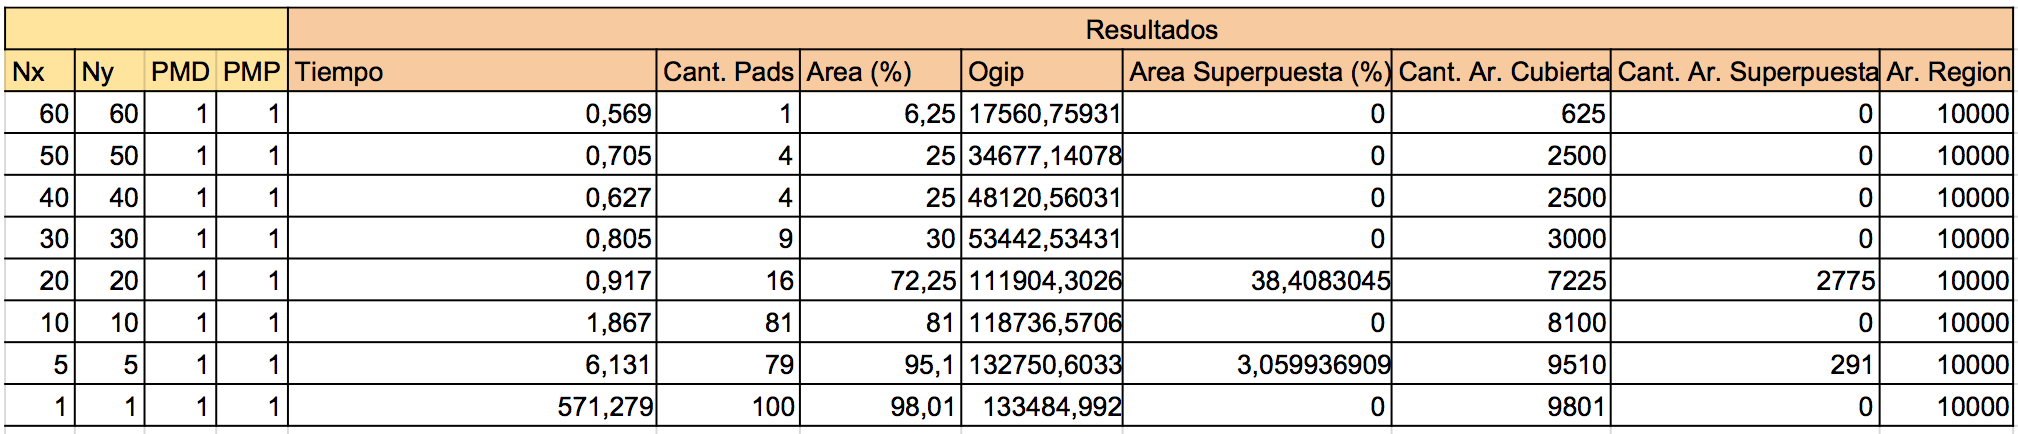
\includegraphics[width=1\textwidth]{imagenes/S_0G100x100_muchos}
\end{center}

\begin{center}
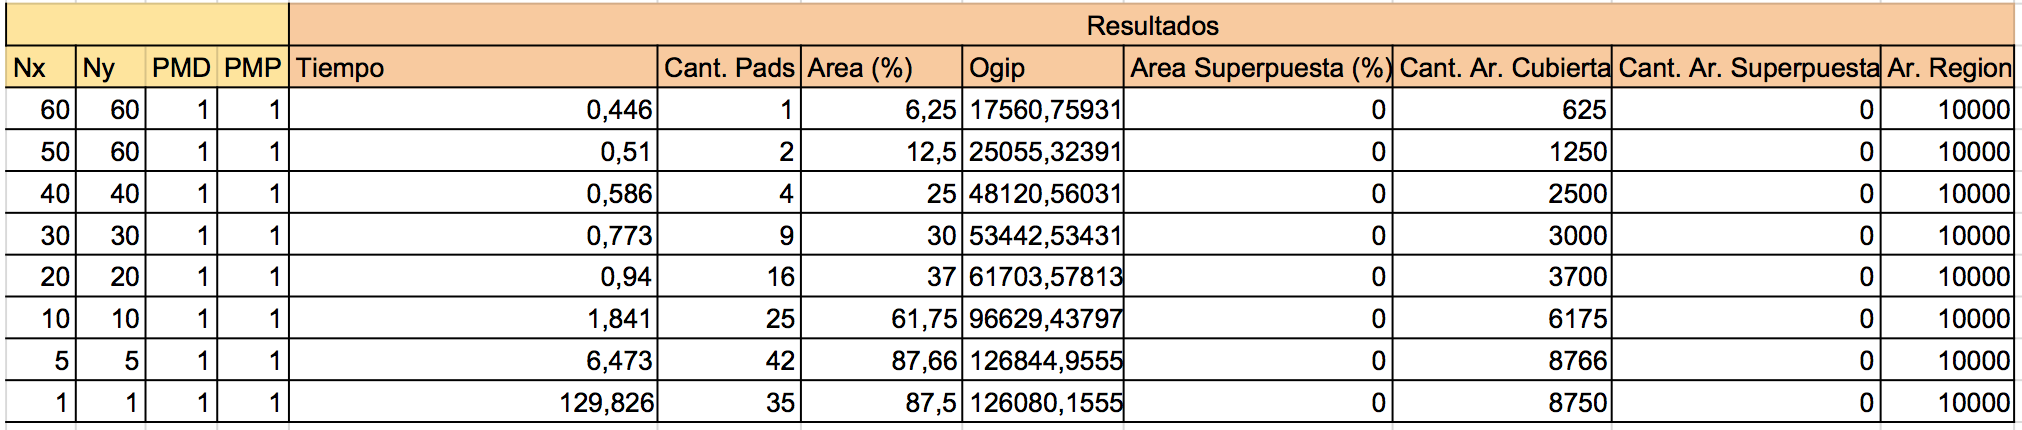
\includegraphics[width=1\textwidth]{imagenes/G_0G100x100_muchos}
\end{center}

\begin{center}
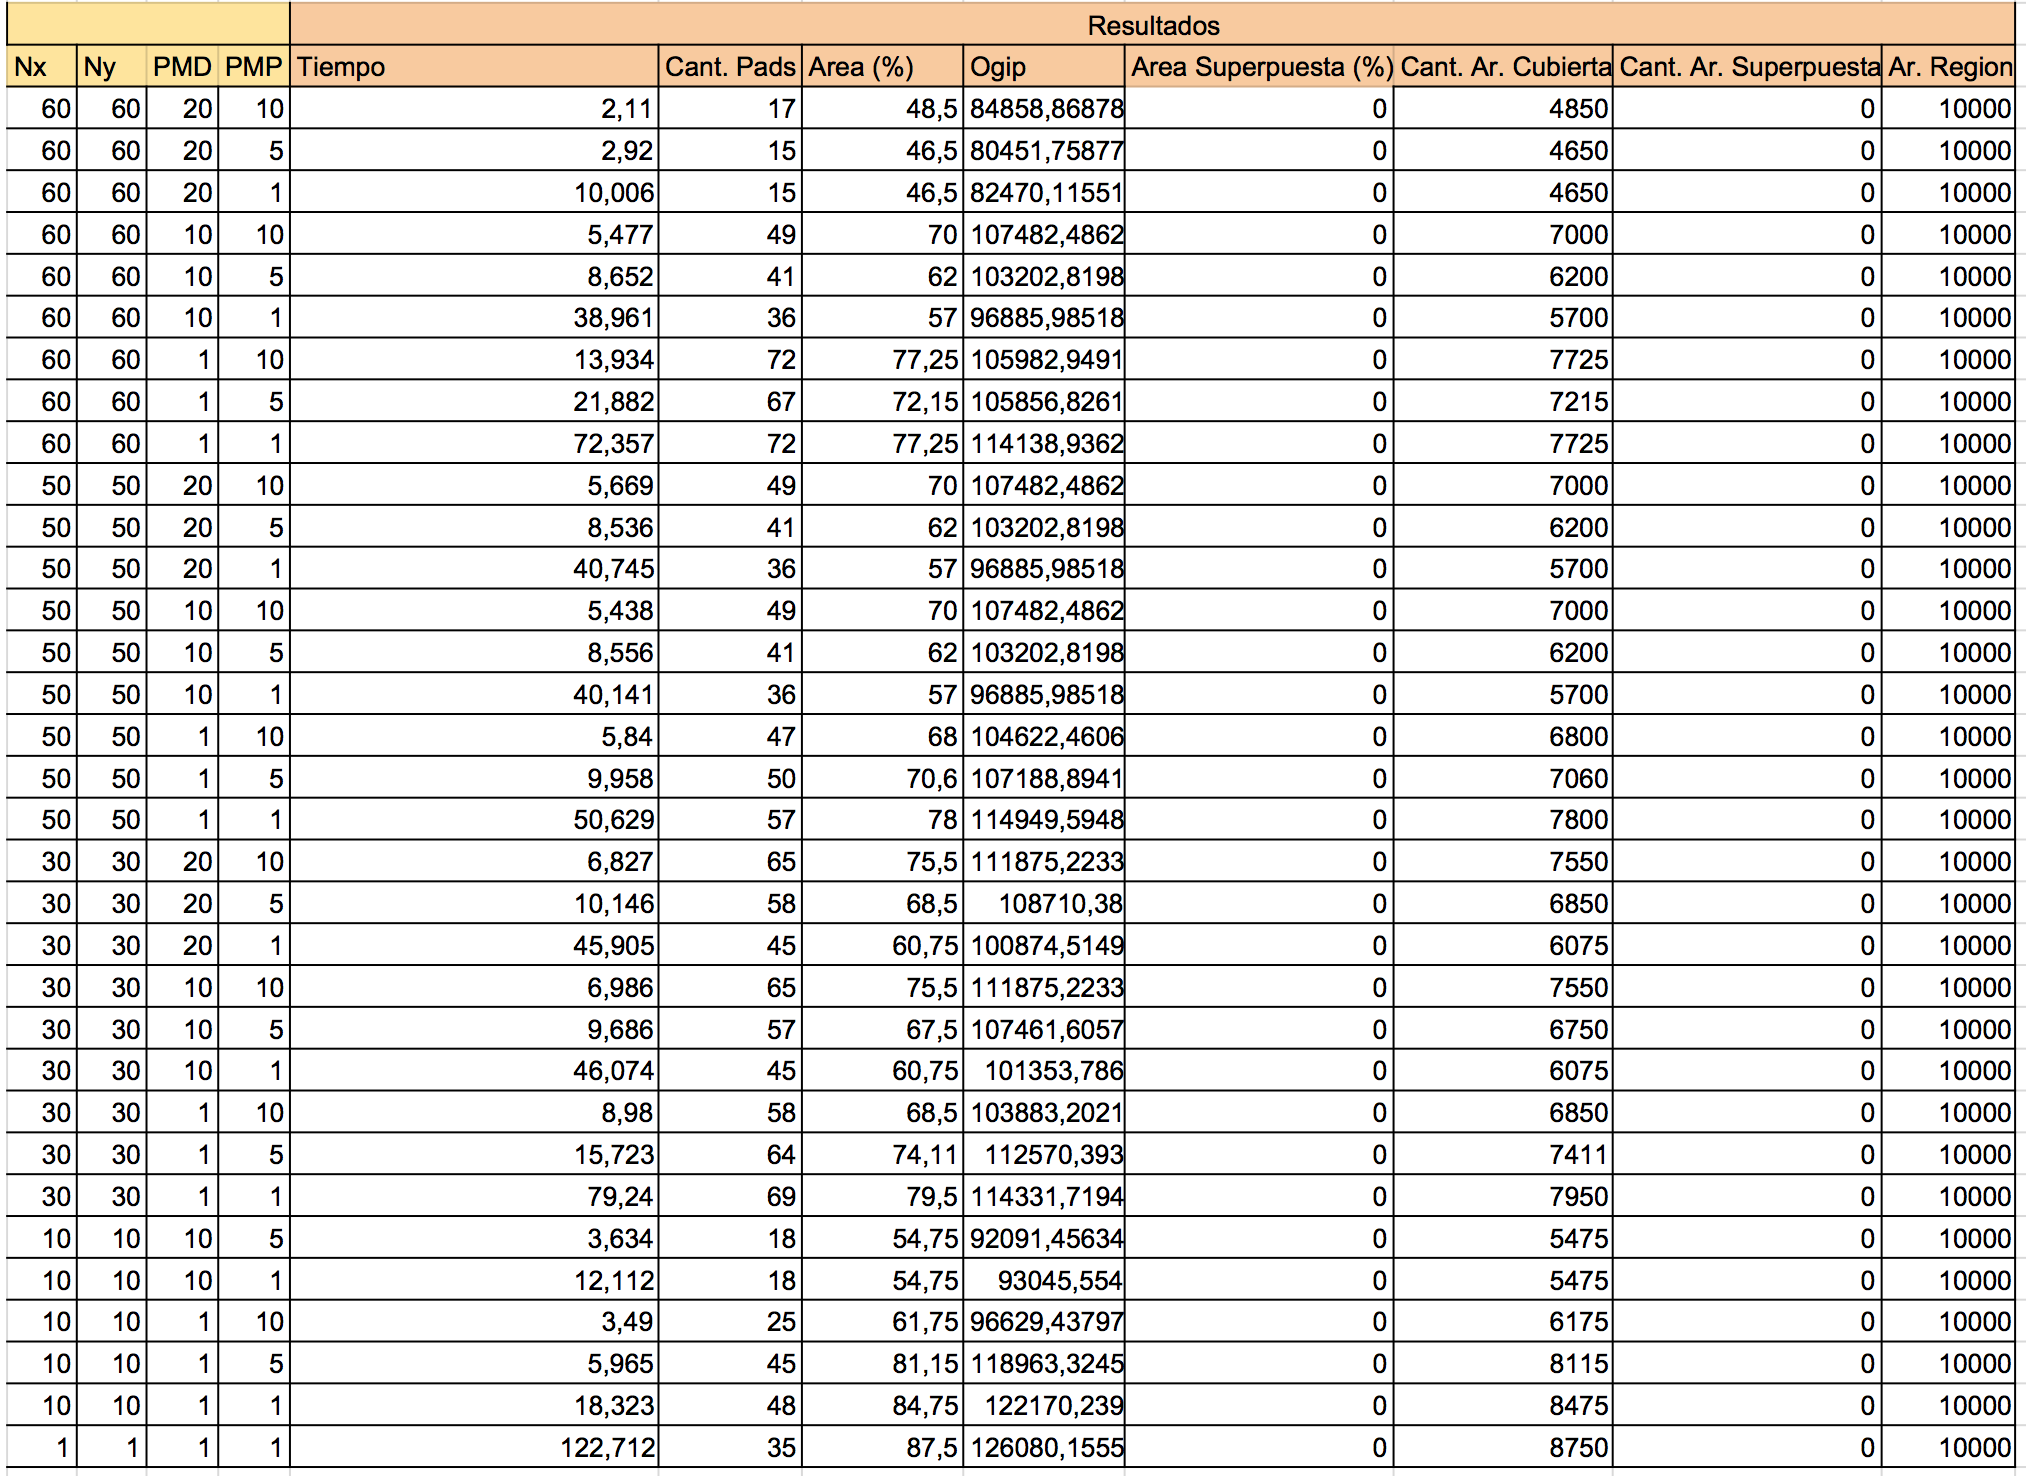
\includegraphics[width=1\textwidth]{imagenes/GML_0G100x100_muchos}
\end{center}


\subsection{0G100x100\_pocos}

\begin{center}
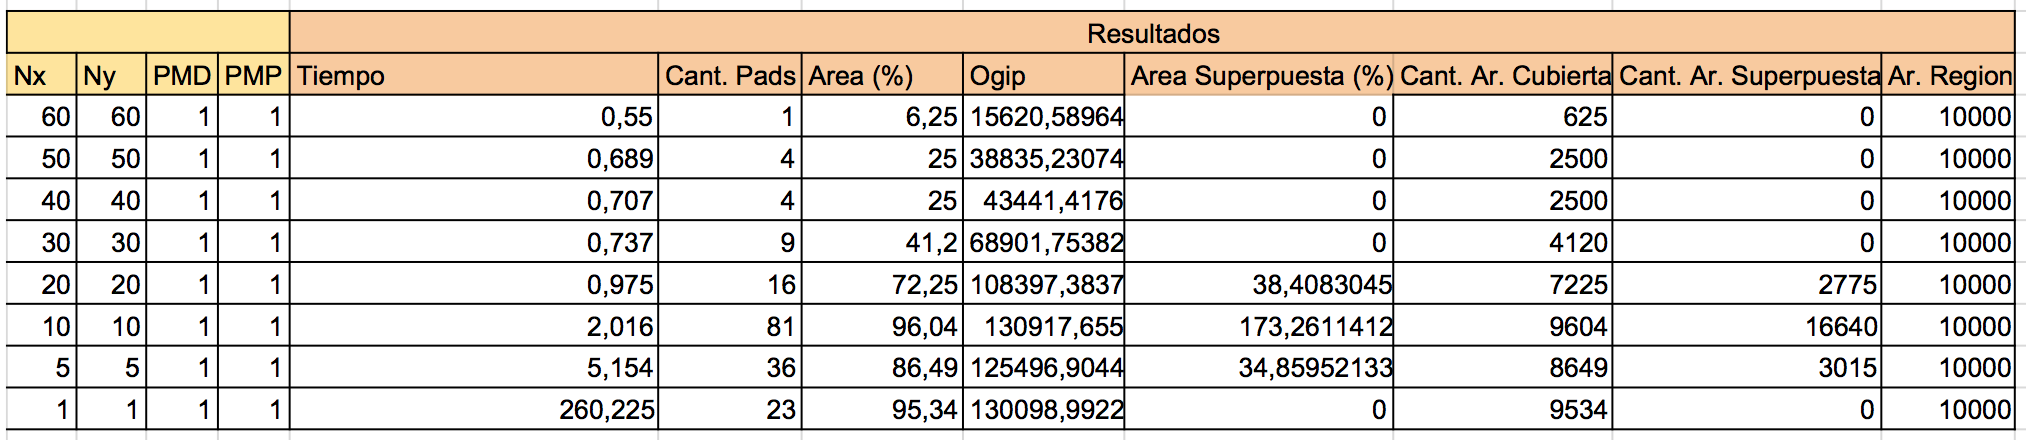
\includegraphics[width=1\textwidth]{imagenes/S_0G100x100_pocos}
\end{center}

\begin{center}
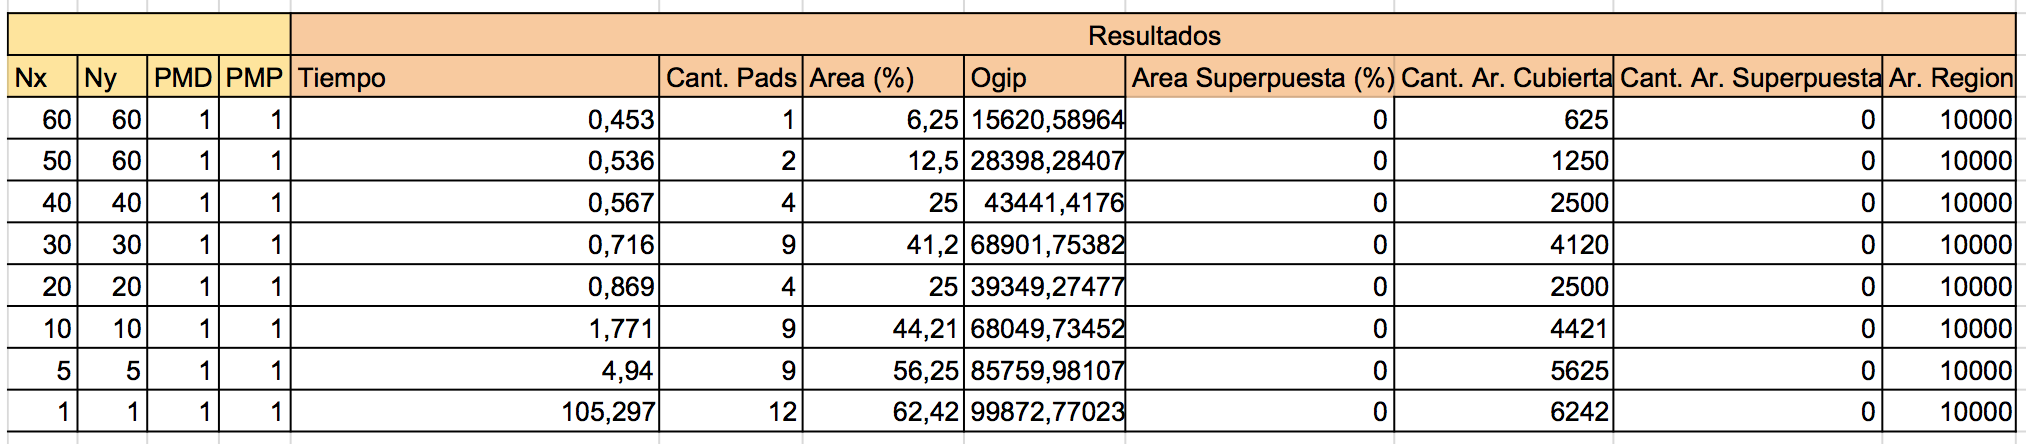
\includegraphics[width=1\textwidth]{imagenes/G_0G100x100_pocos}
\end{center}

\begin{center}
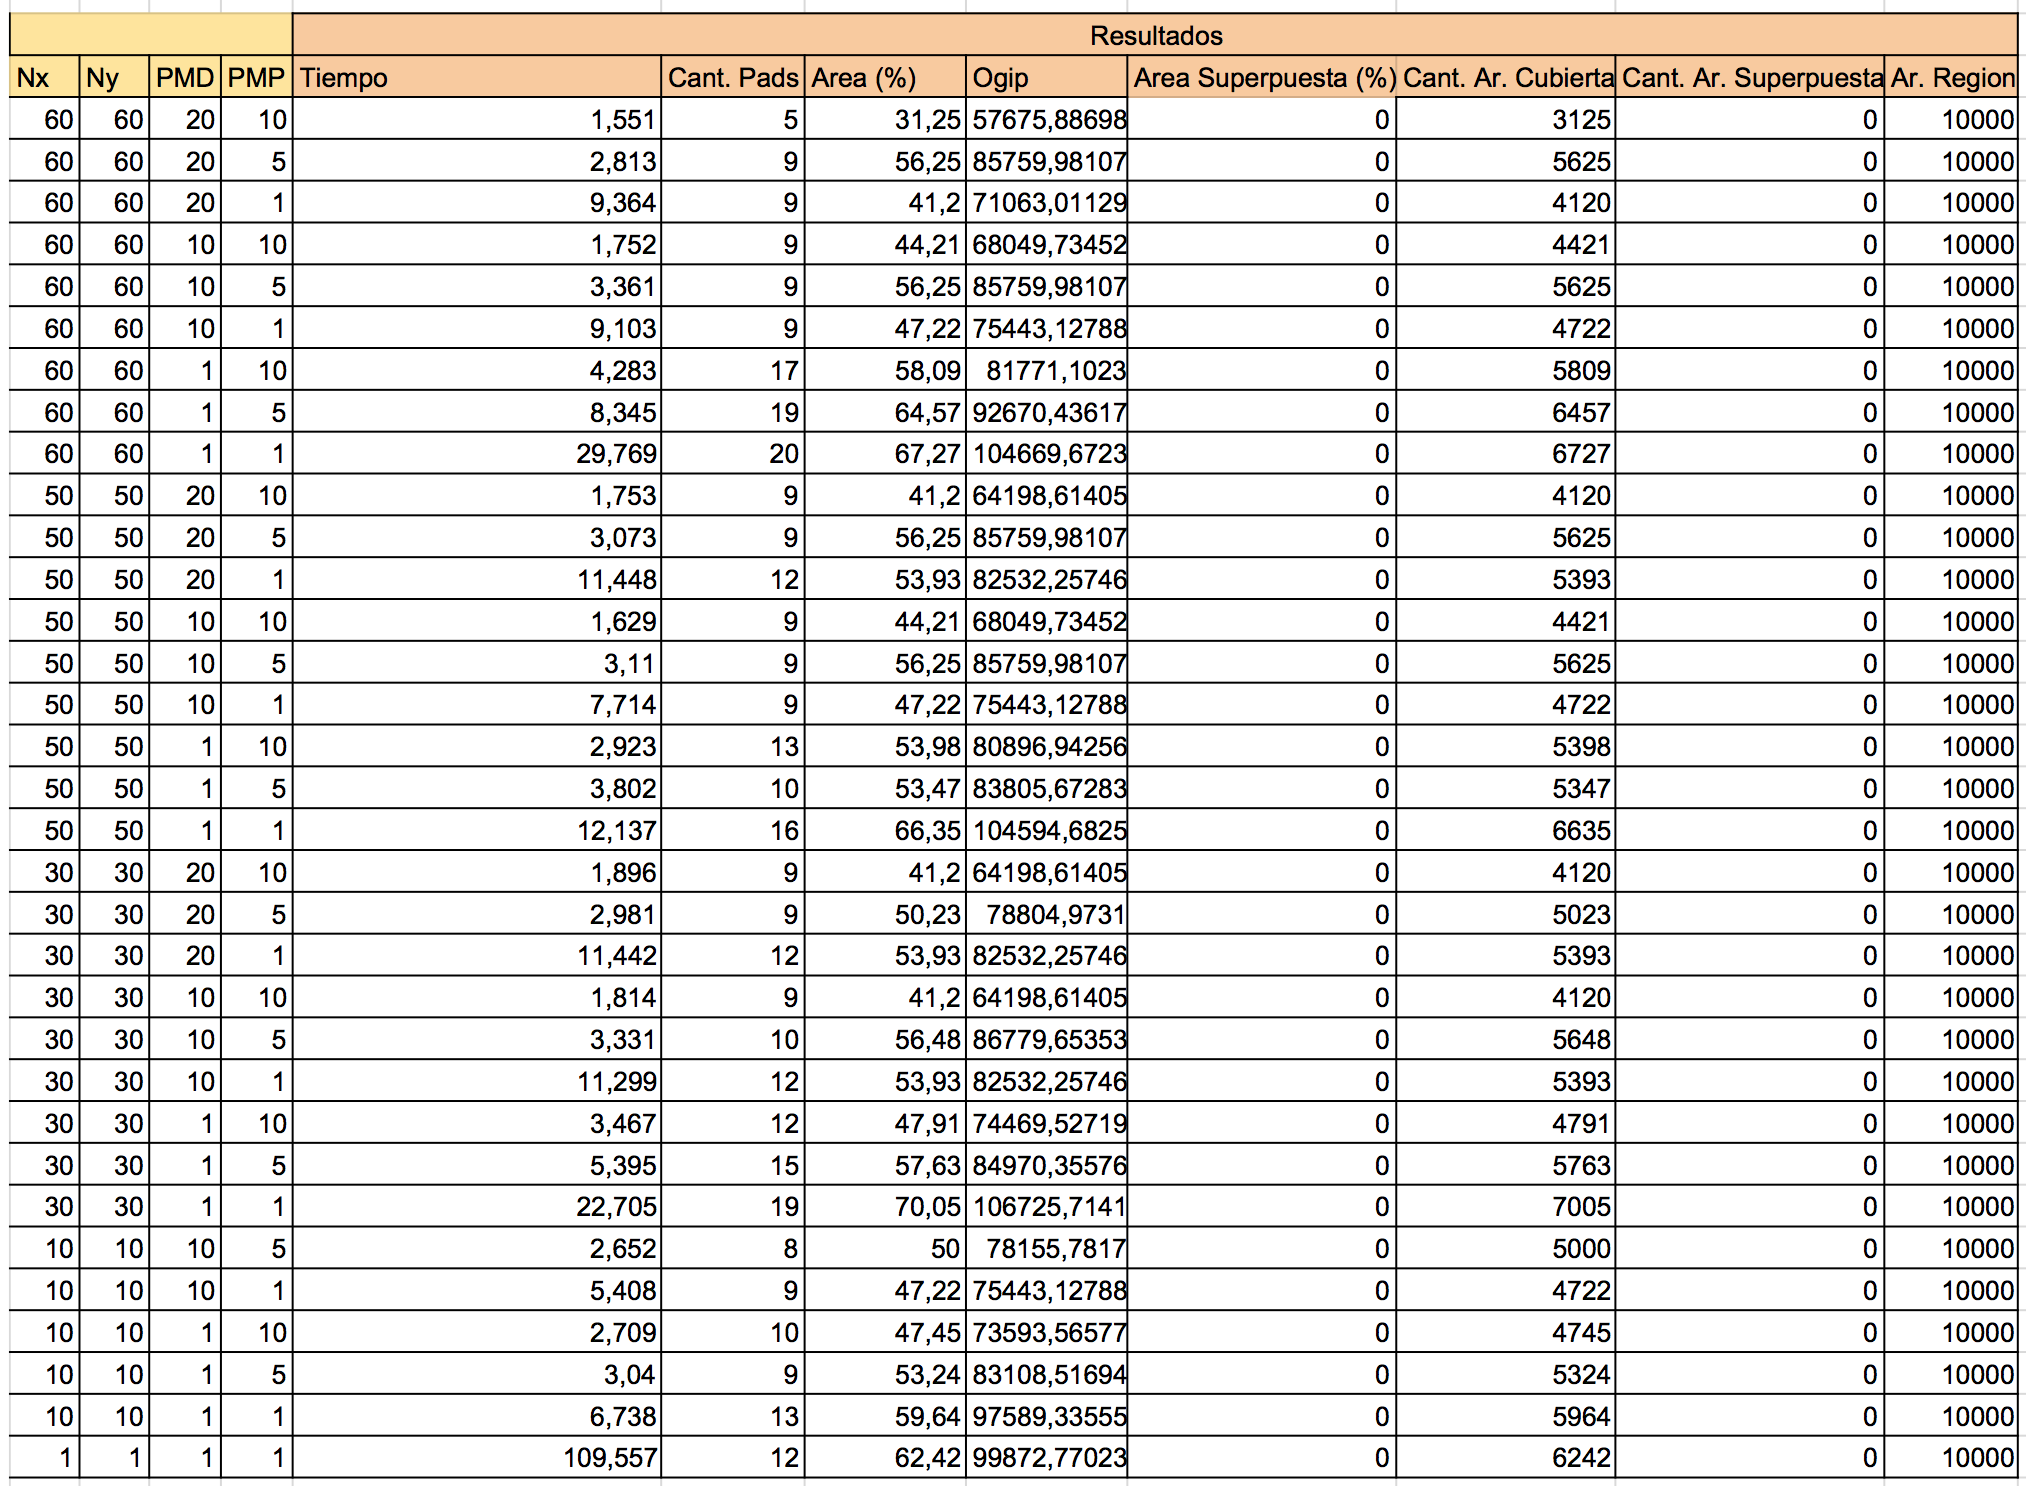
\includegraphics[width=1\textwidth]{imagenes/GML_0G100x100_pocos}
\end{center}

\subsection{45G100x100\_pocos}

\begin{center}
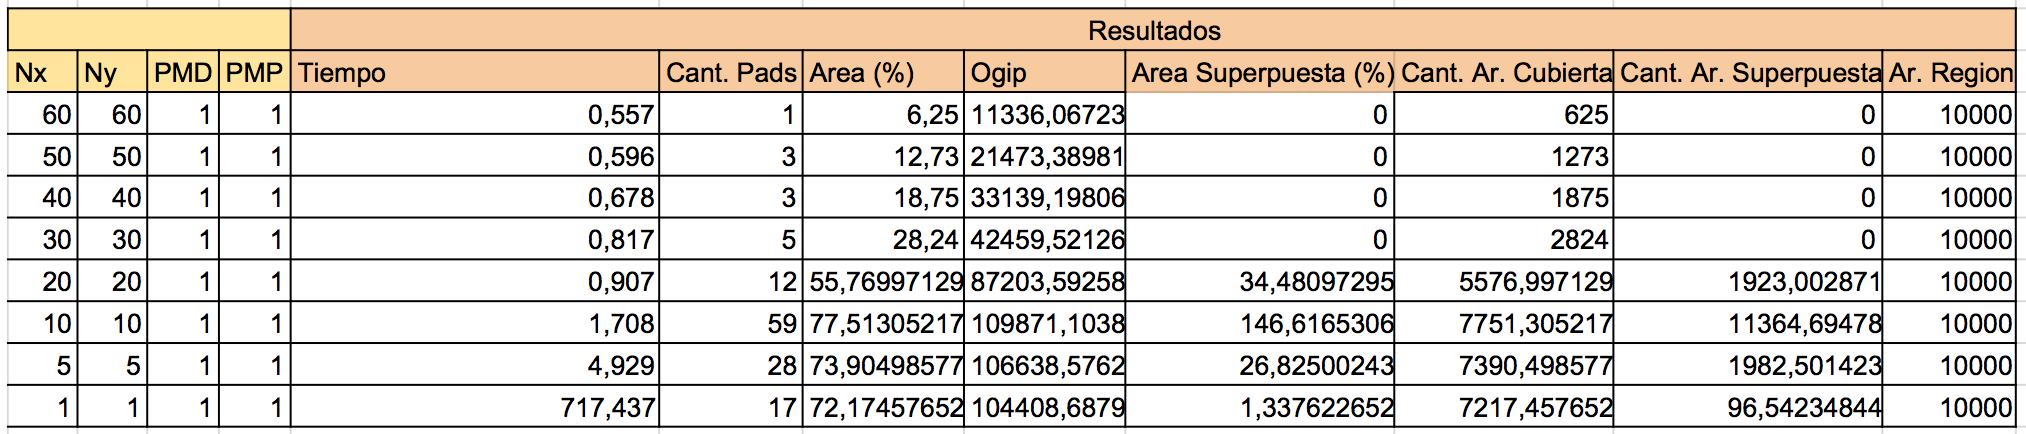
\includegraphics[width=1\textwidth]{imagenes/S_45G100x100_pocos}
\end{center}

\begin{center}
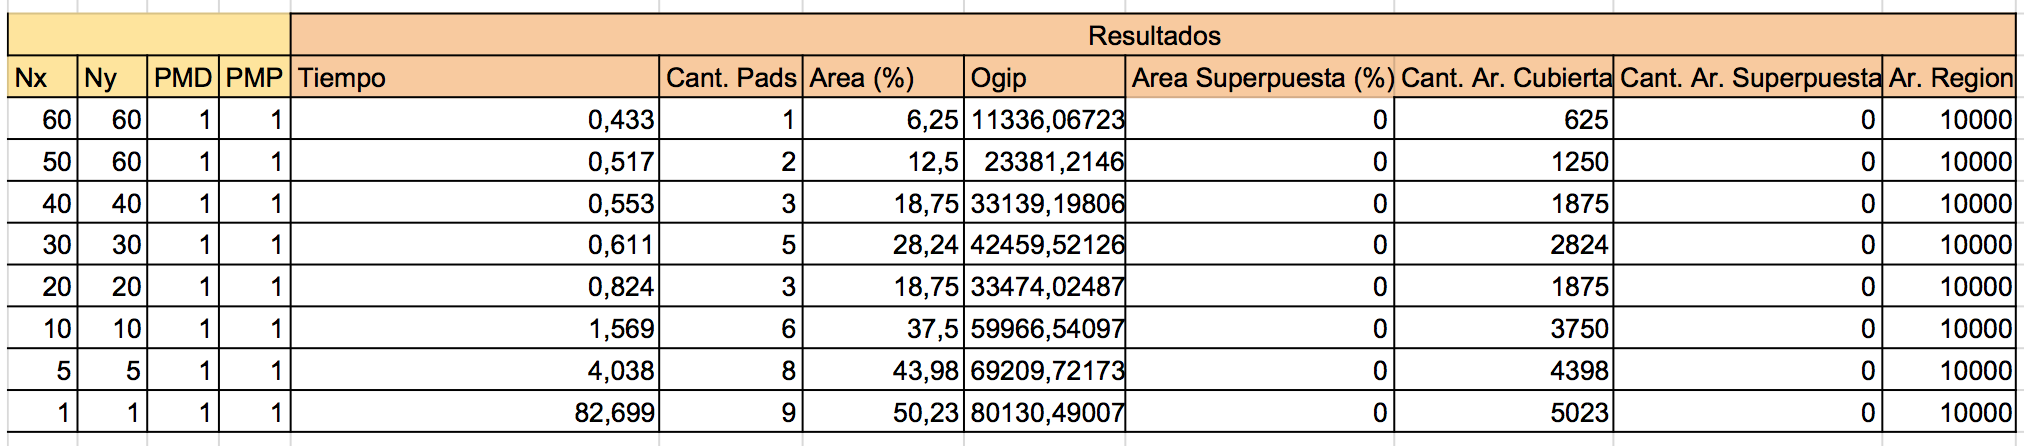
\includegraphics[width=1\textwidth]{imagenes/G_45G100x100_pocos}
\end{center}

\begin{center}
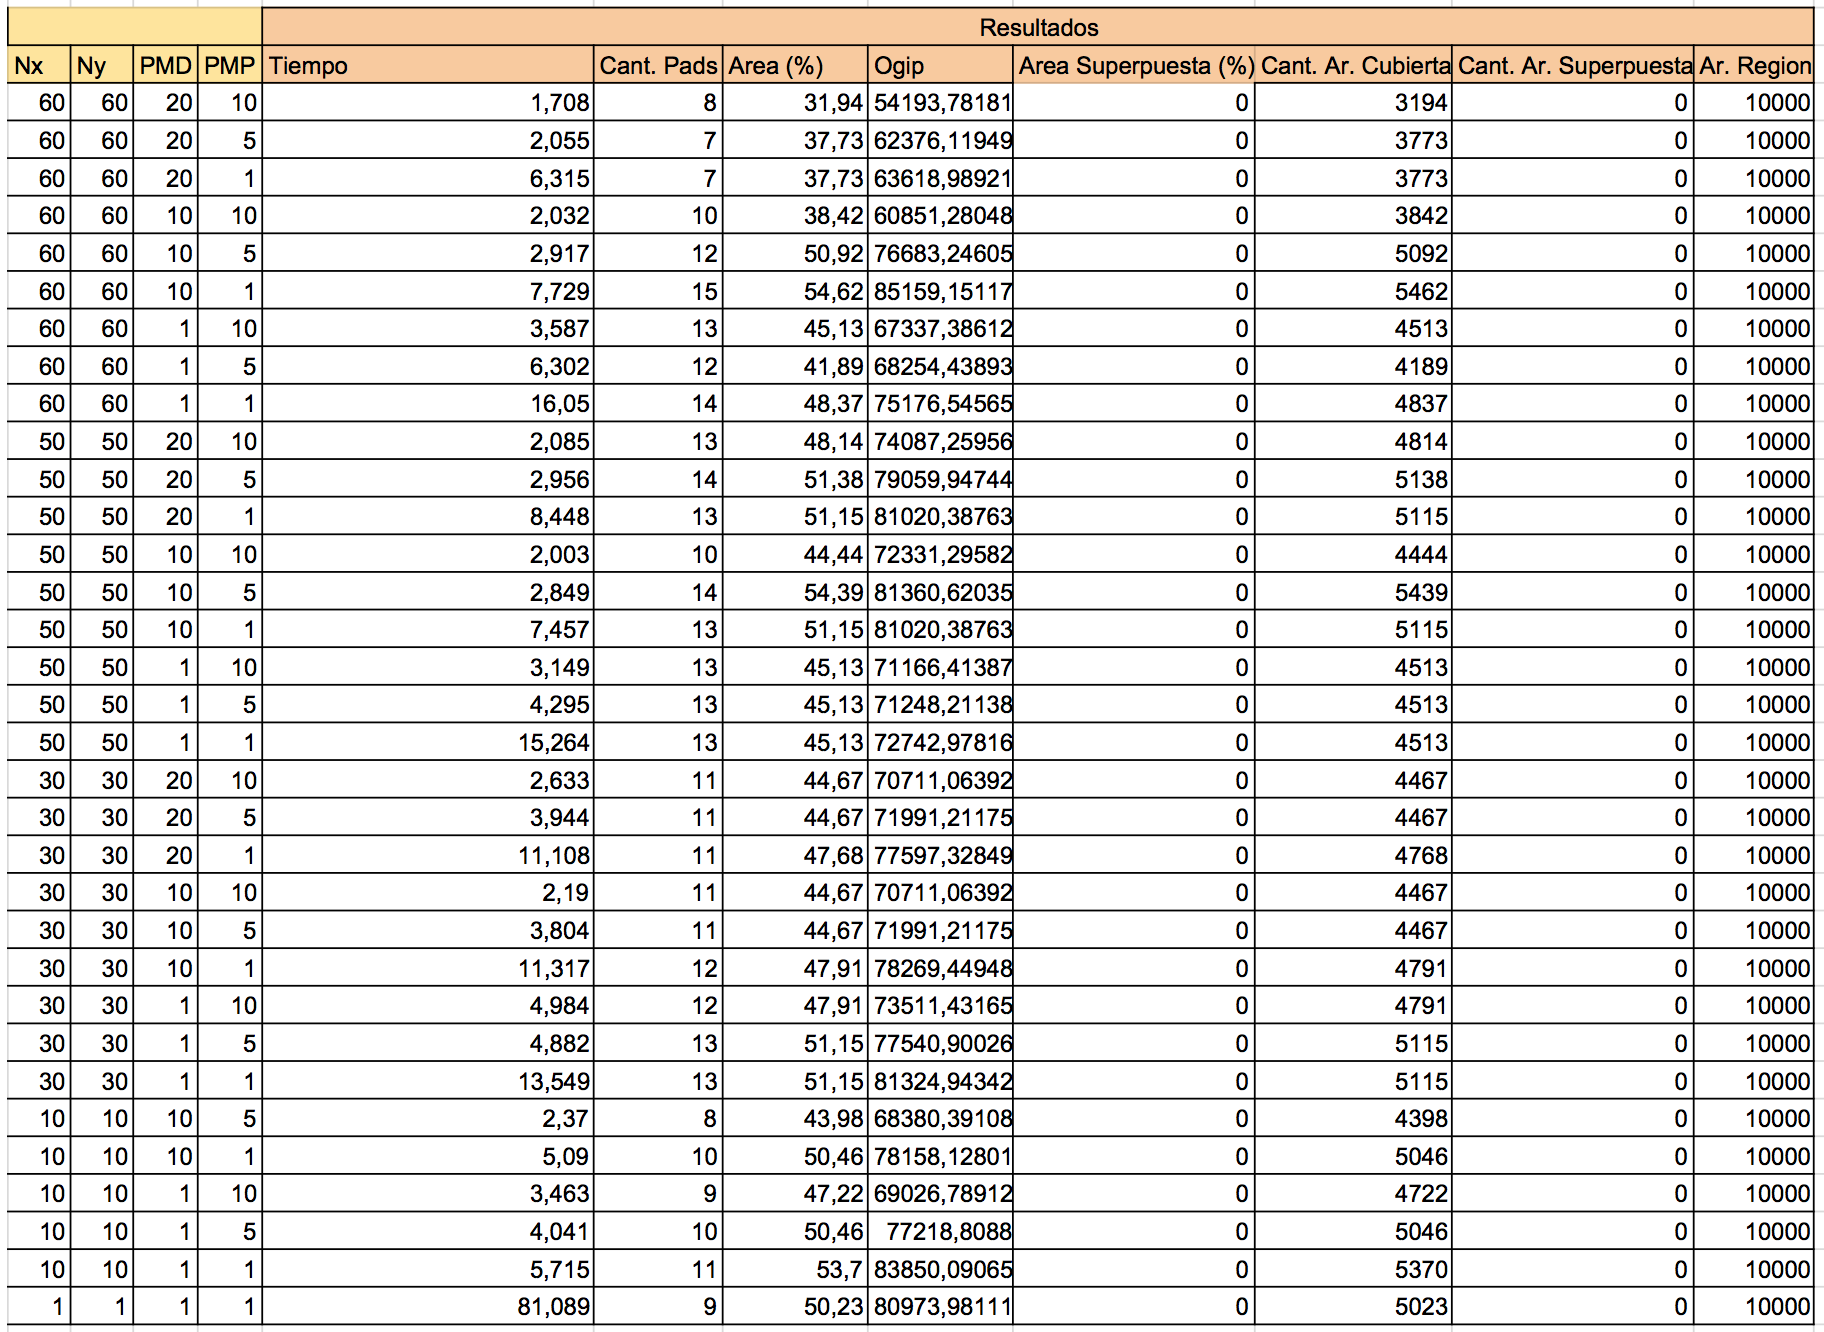
\includegraphics[width=1\textwidth]{imagenes/GML_45G100x100_pocos}
\end{center}

\subsection{45G100x100\_muchos}

\begin{center}
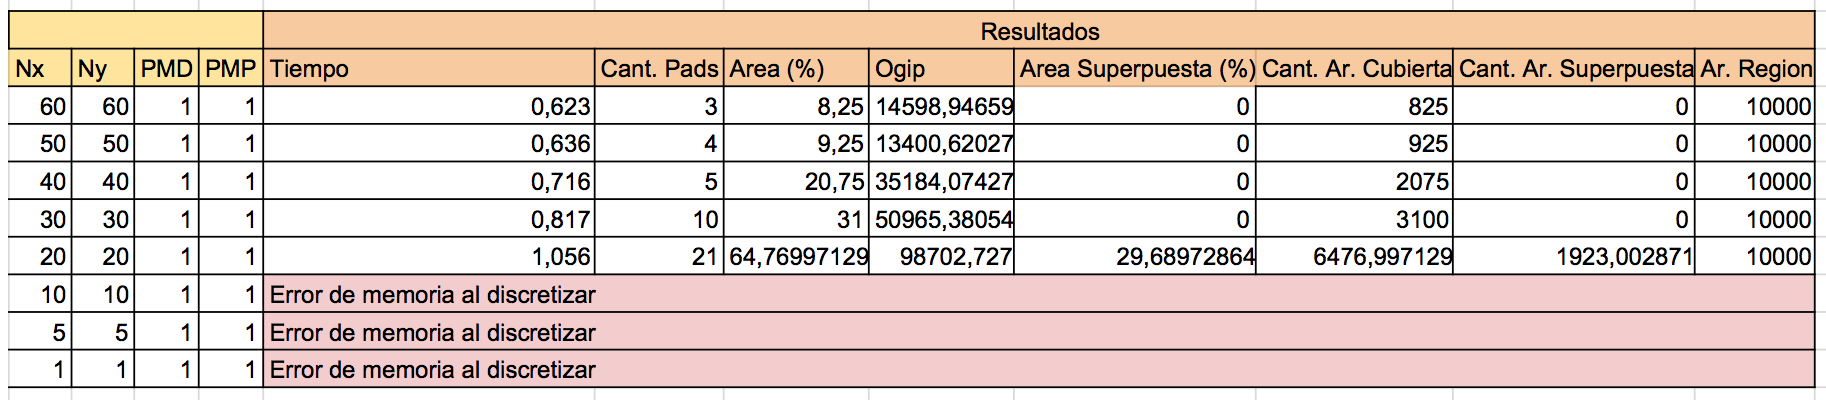
\includegraphics[width=1\textwidth]{imagenes/S_45G100x100_muchos}
\end{center}

\begin{center}
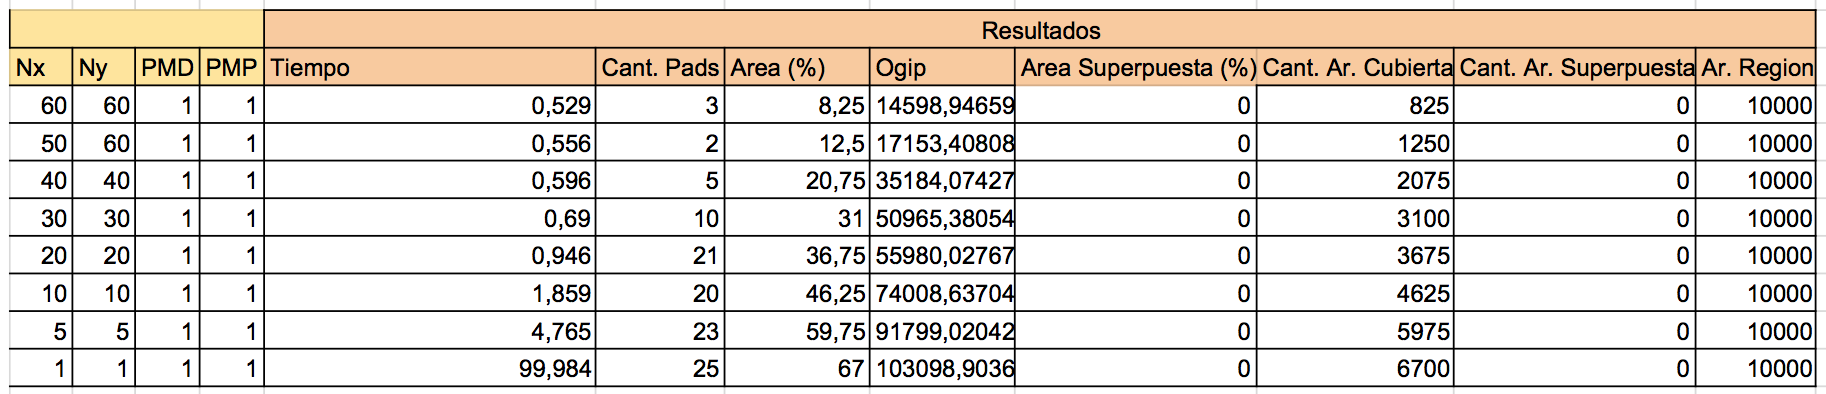
\includegraphics[width=1\textwidth]{imagenes/G_45G100x100_muchos}
\end{center}

\begin{center}
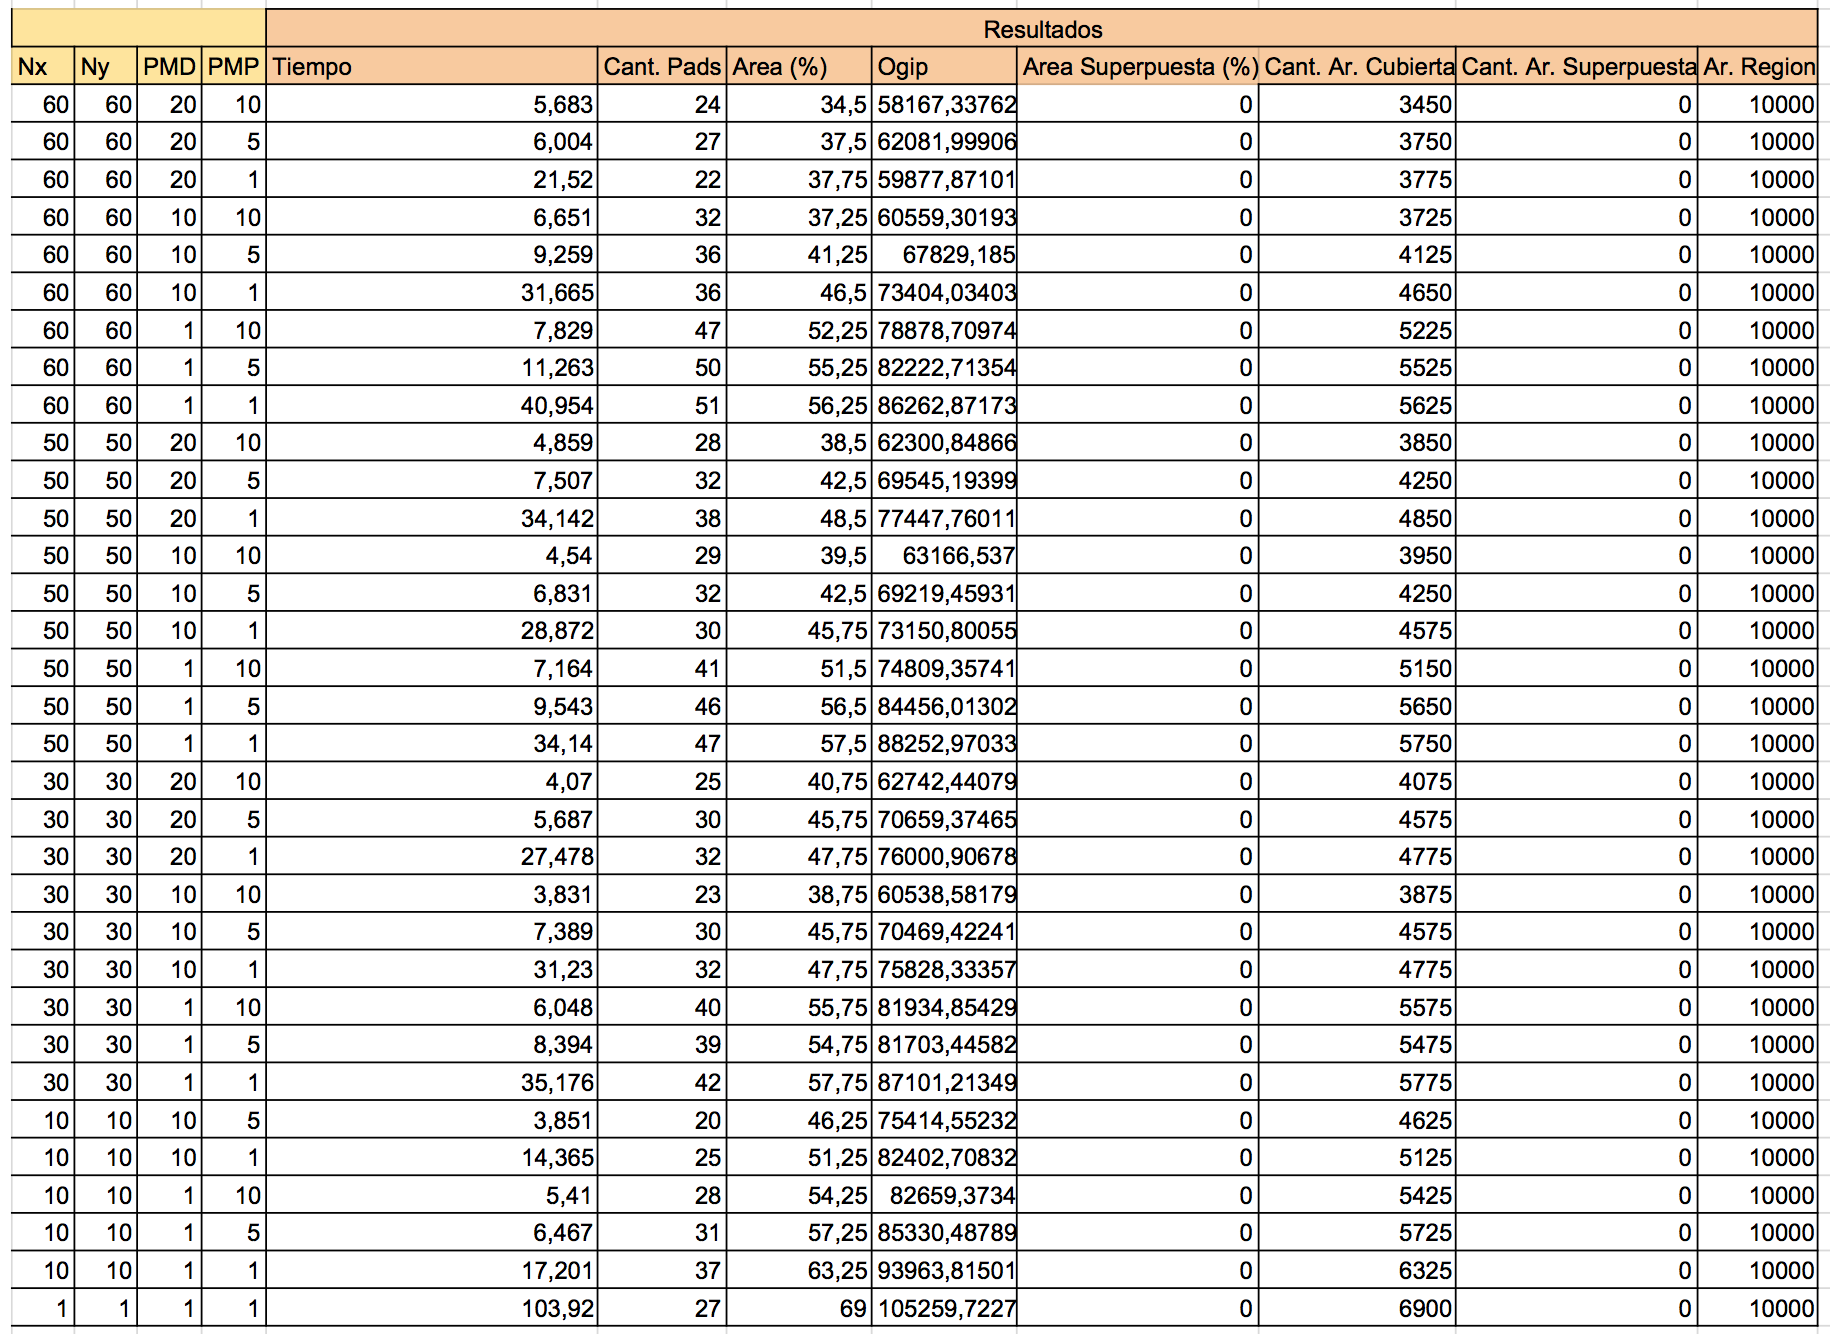
\includegraphics[width=1\textwidth]{imagenes/GML_45G100x100_muchos}
\end{center}

\subsection{0G400x400\_pocos}

\begin{center}
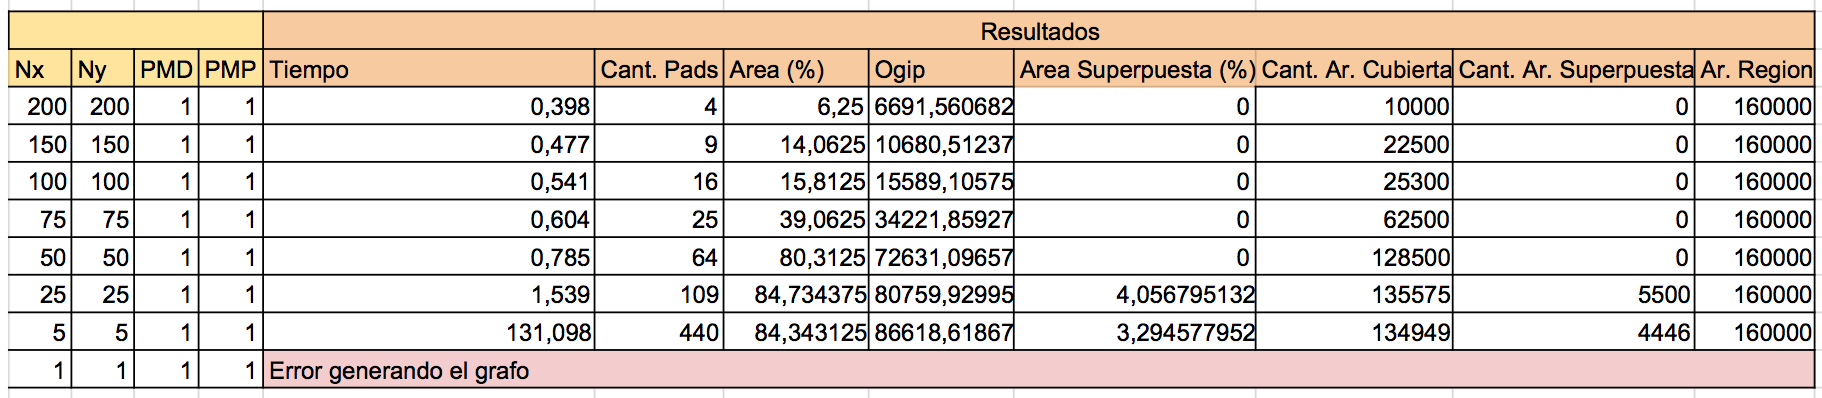
\includegraphics[width=1\textwidth]{imagenes/S_0G400x400_pocos}
\end{center}

\begin{center}
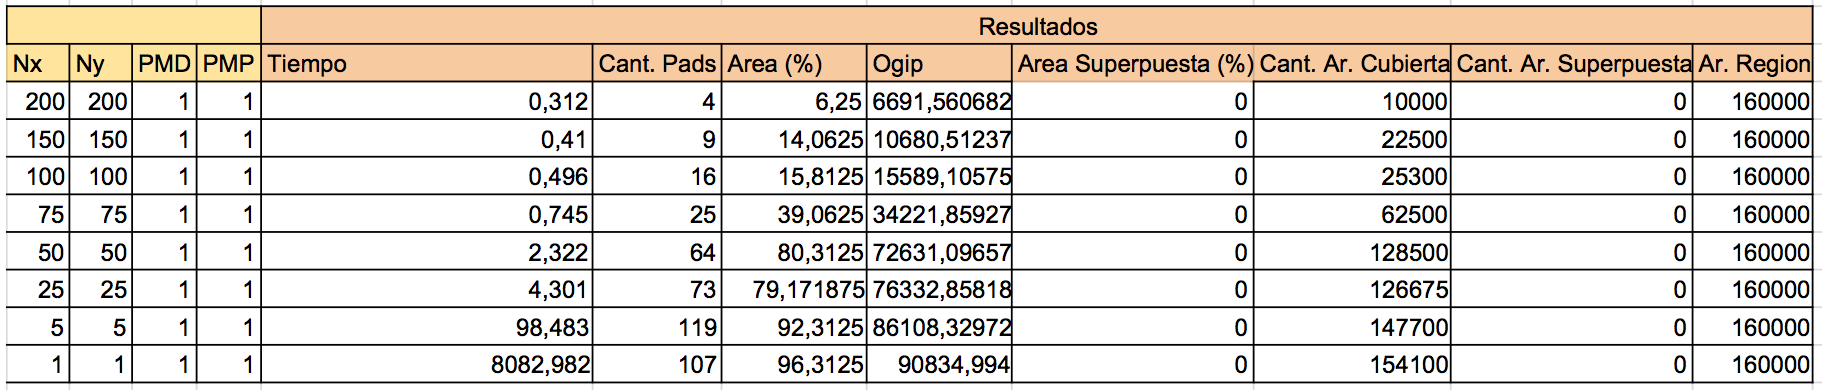
\includegraphics[width=1\textwidth]{imagenes/G_0G400x400_pocos}
\end{center}

\begin{center}
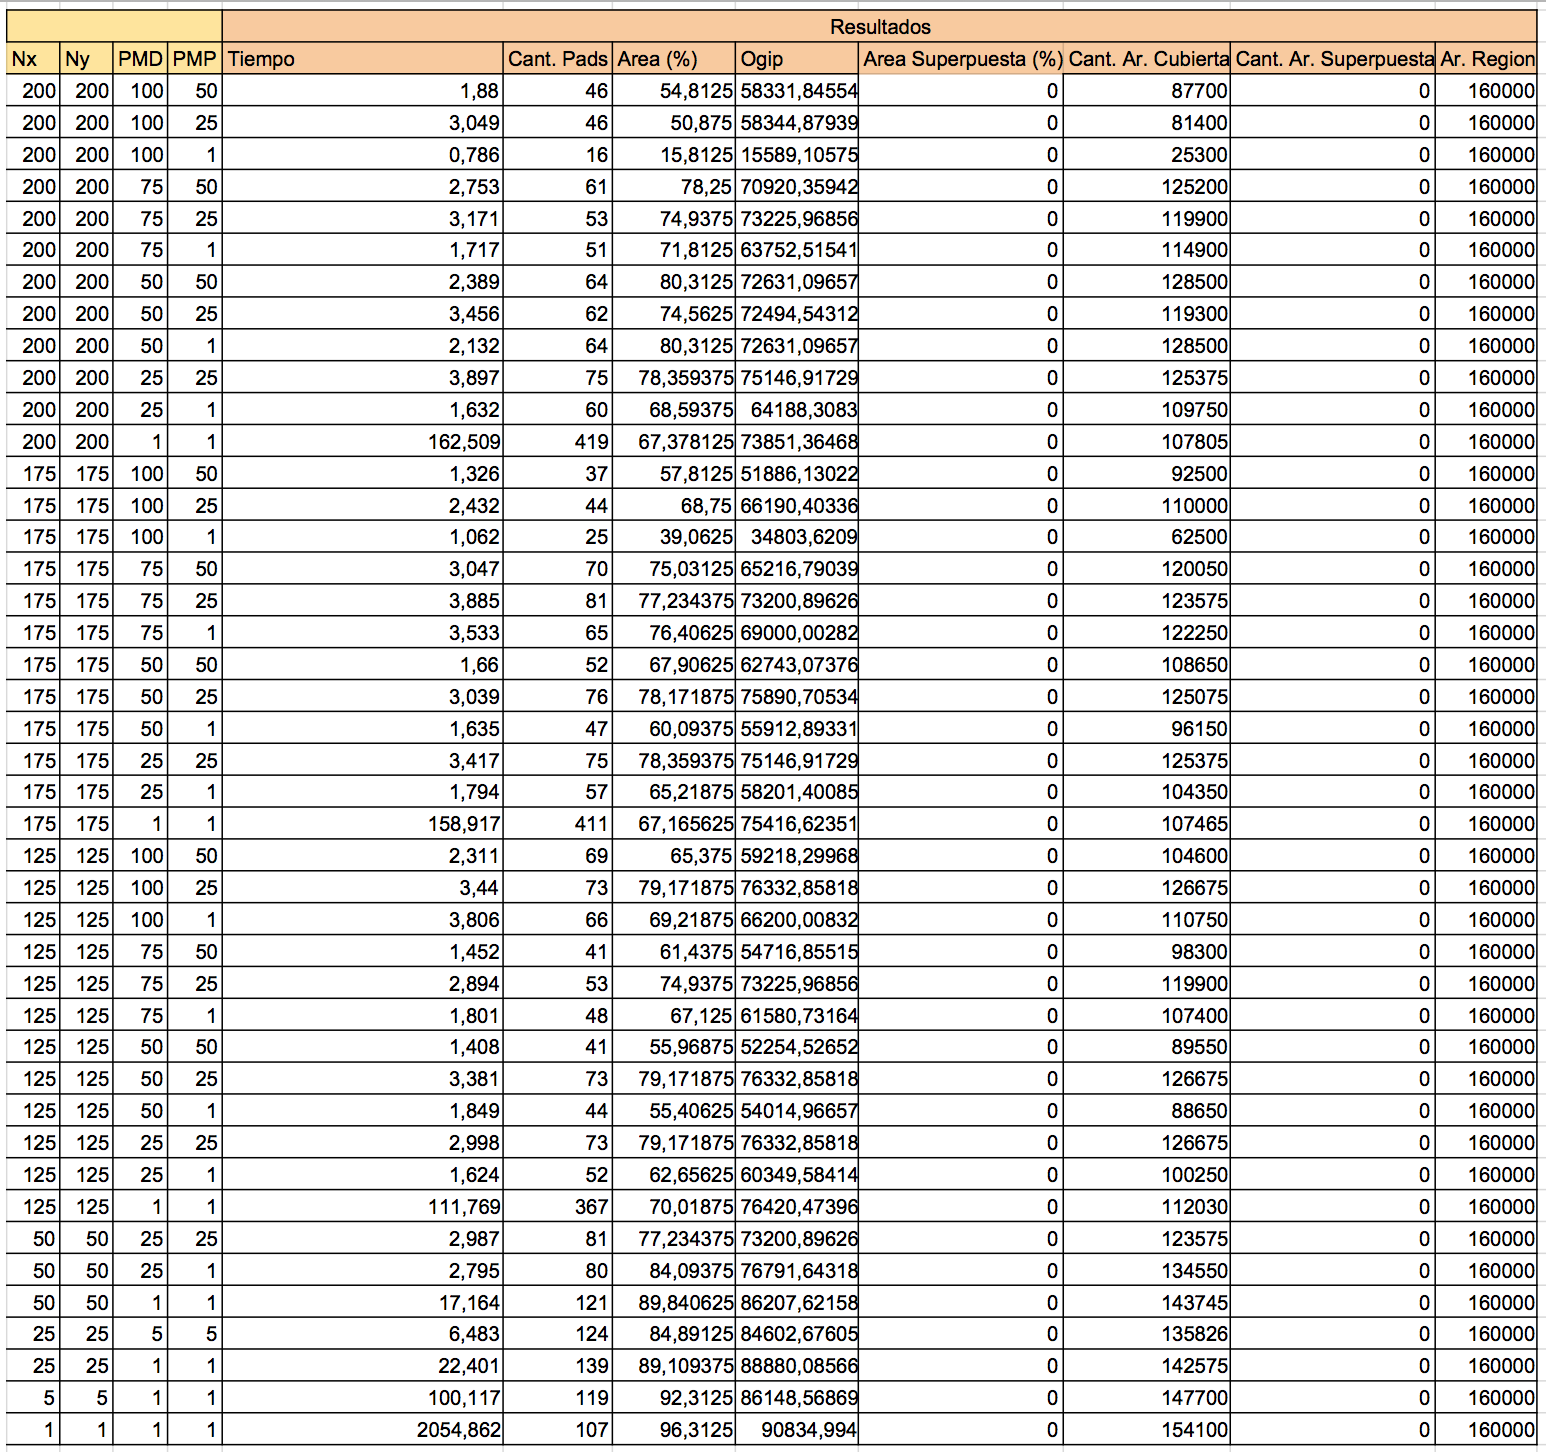
\includegraphics[width=1\textwidth]{imagenes/GML_0G400x400_pocos}
\end{center}

\subsection{45G400x400\_pocos}

\begin{center}
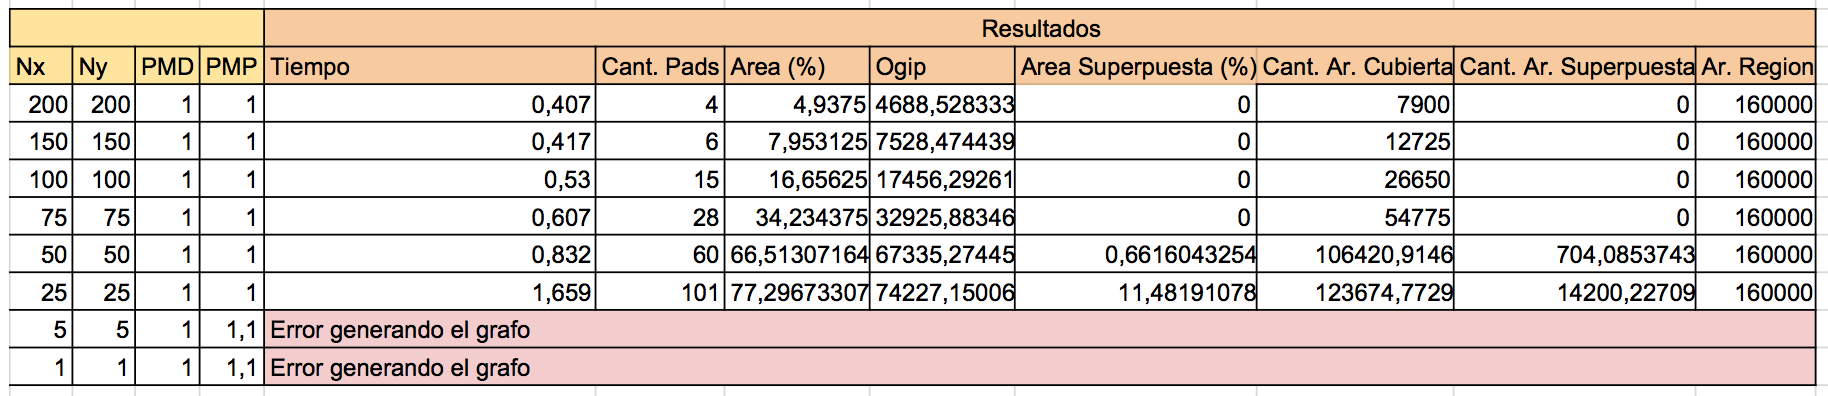
\includegraphics[width=1\textwidth]{imagenes/S_45G400x400_pocos}
\end{center}

\begin{center}
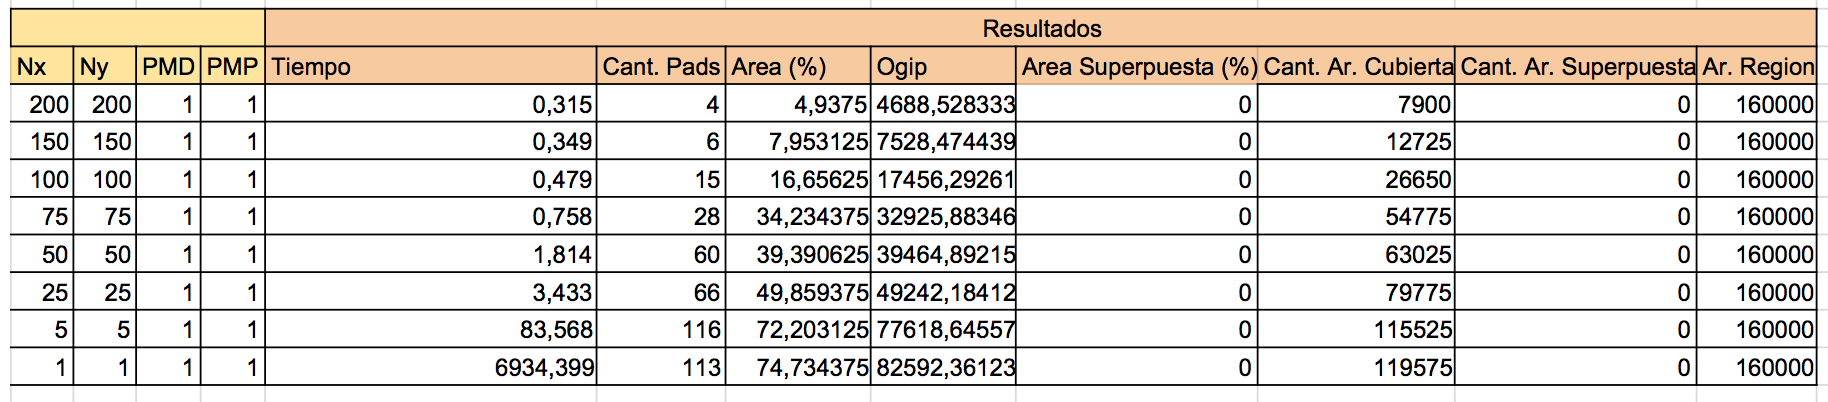
\includegraphics[width=1\textwidth]{imagenes/G_45G400x400_pocos}
\end{center}

\begin{center}
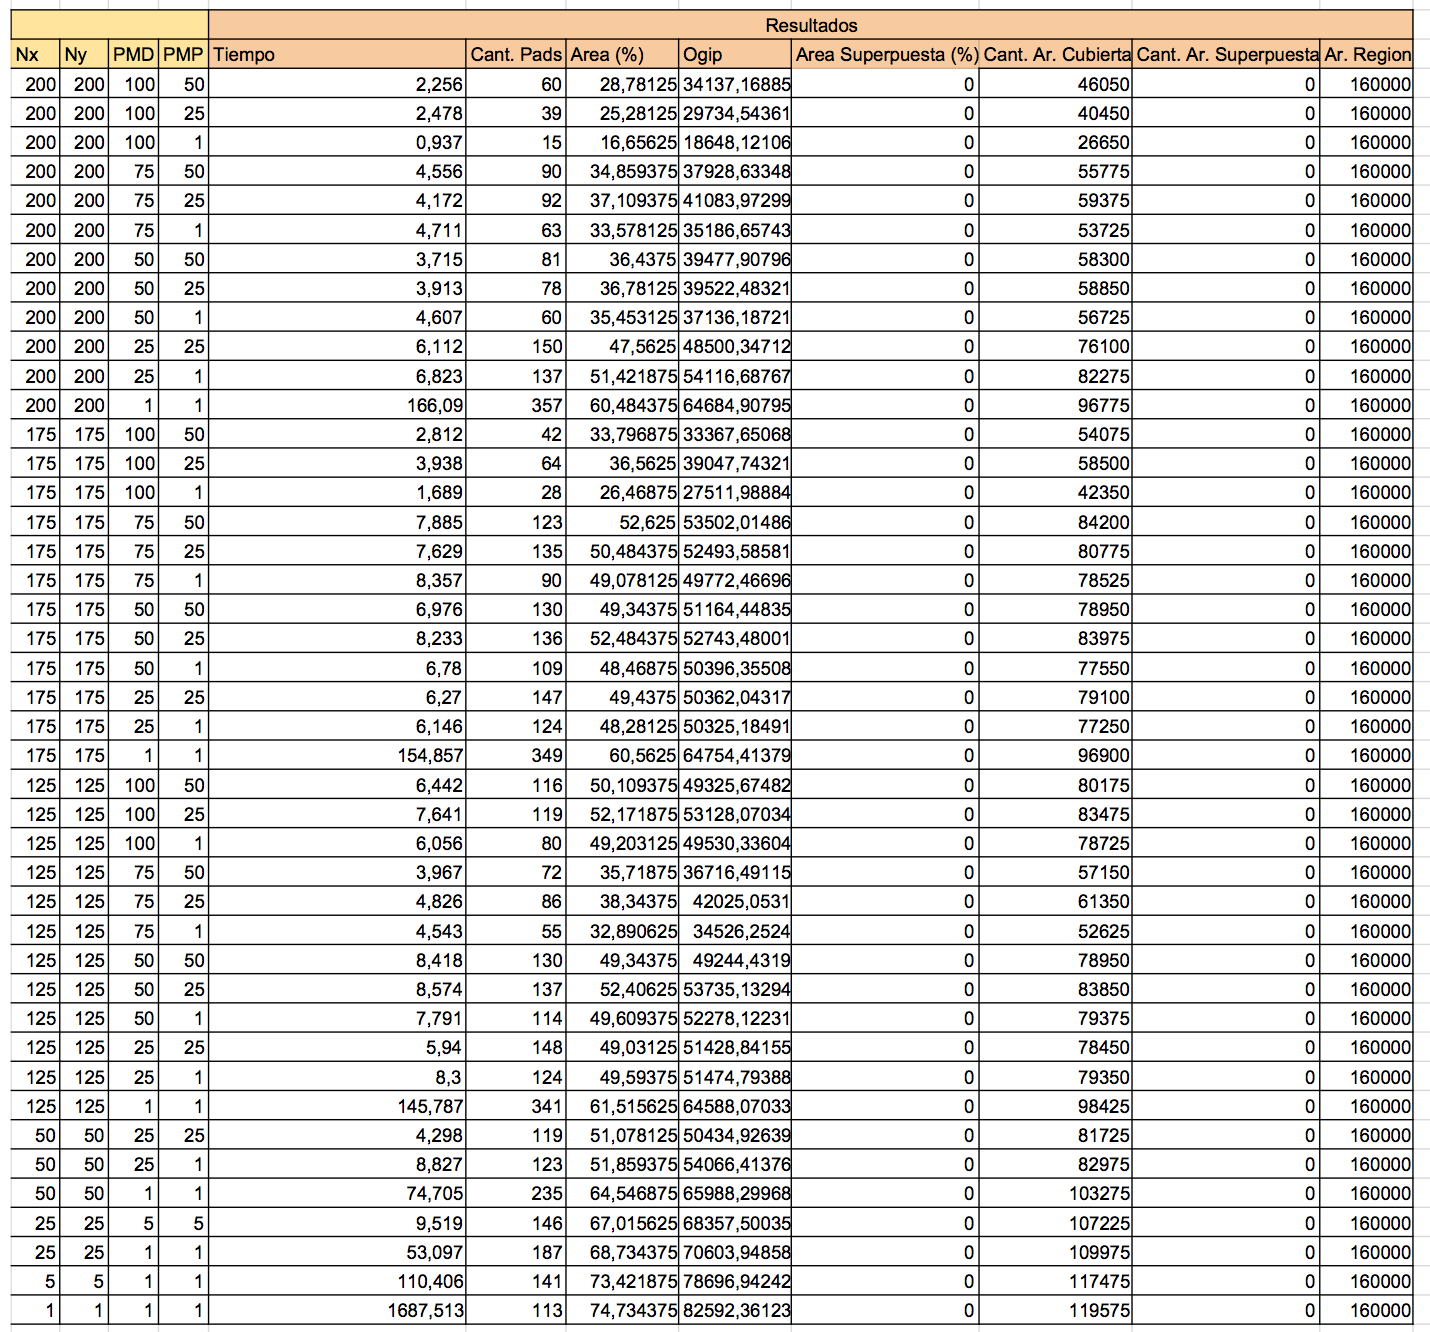
\includegraphics[width=1\textwidth]{imagenes/GML_45G400x400_pocos}
\end{center}

\subsection{inst2}

\begin{center}
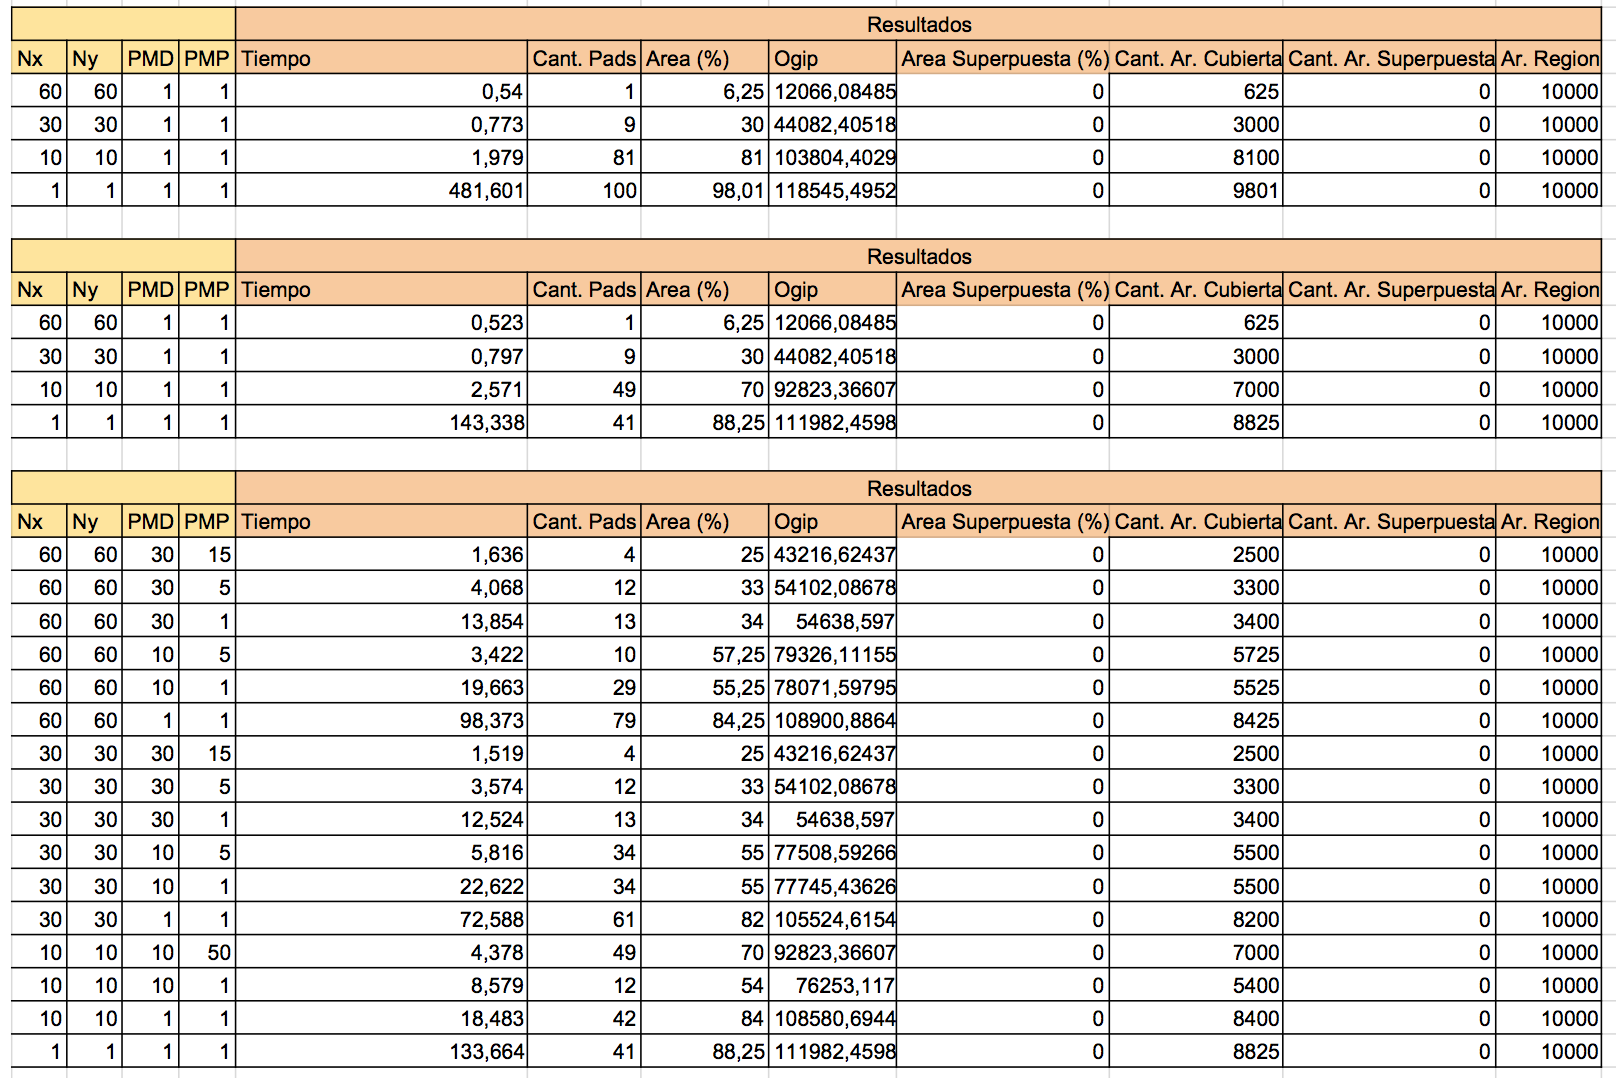
\includegraphics[width=1\textwidth]{imagenes/ALL_inst2}
\end{center}

\subsection{0G1200x1200\_muchos}


\begin{center}
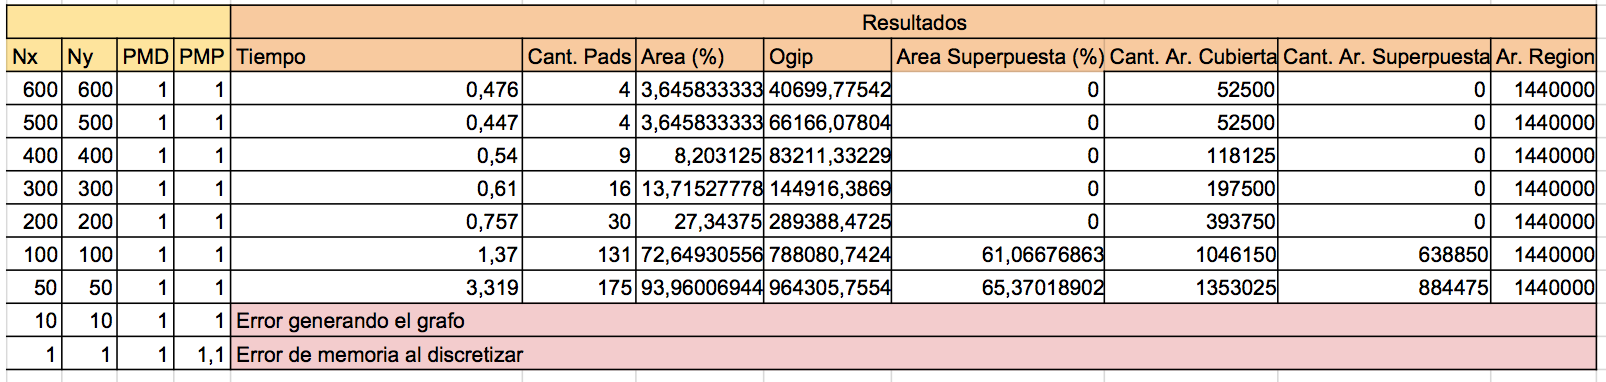
\includegraphics[width=1\textwidth]{imagenes/S_0G1200x1200_muchos}
\end{center}

\begin{center}
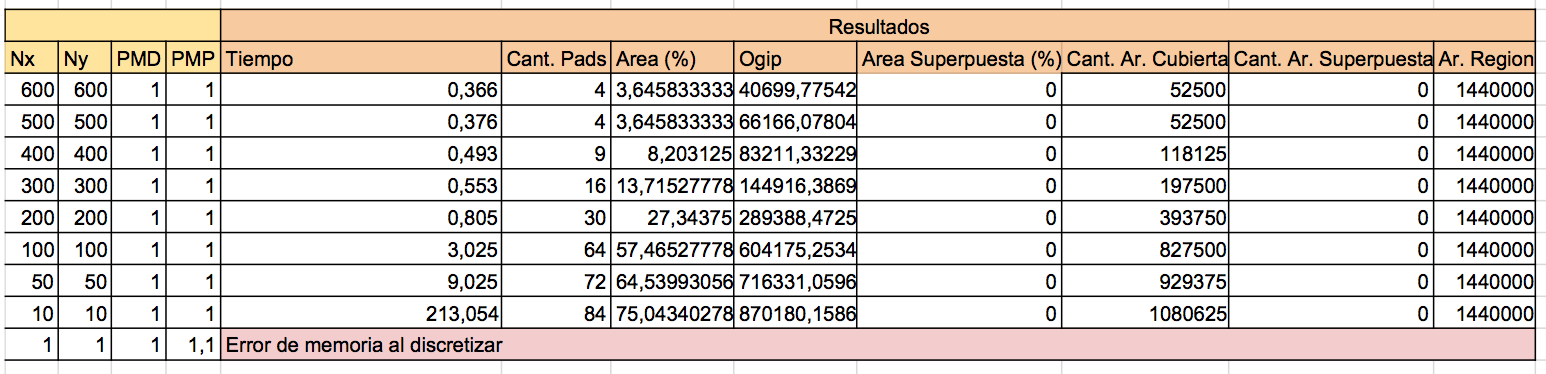
\includegraphics[width=1\textwidth]{imagenes/G_0G1200x1200_muchos}
\end{center}

\begin{center}
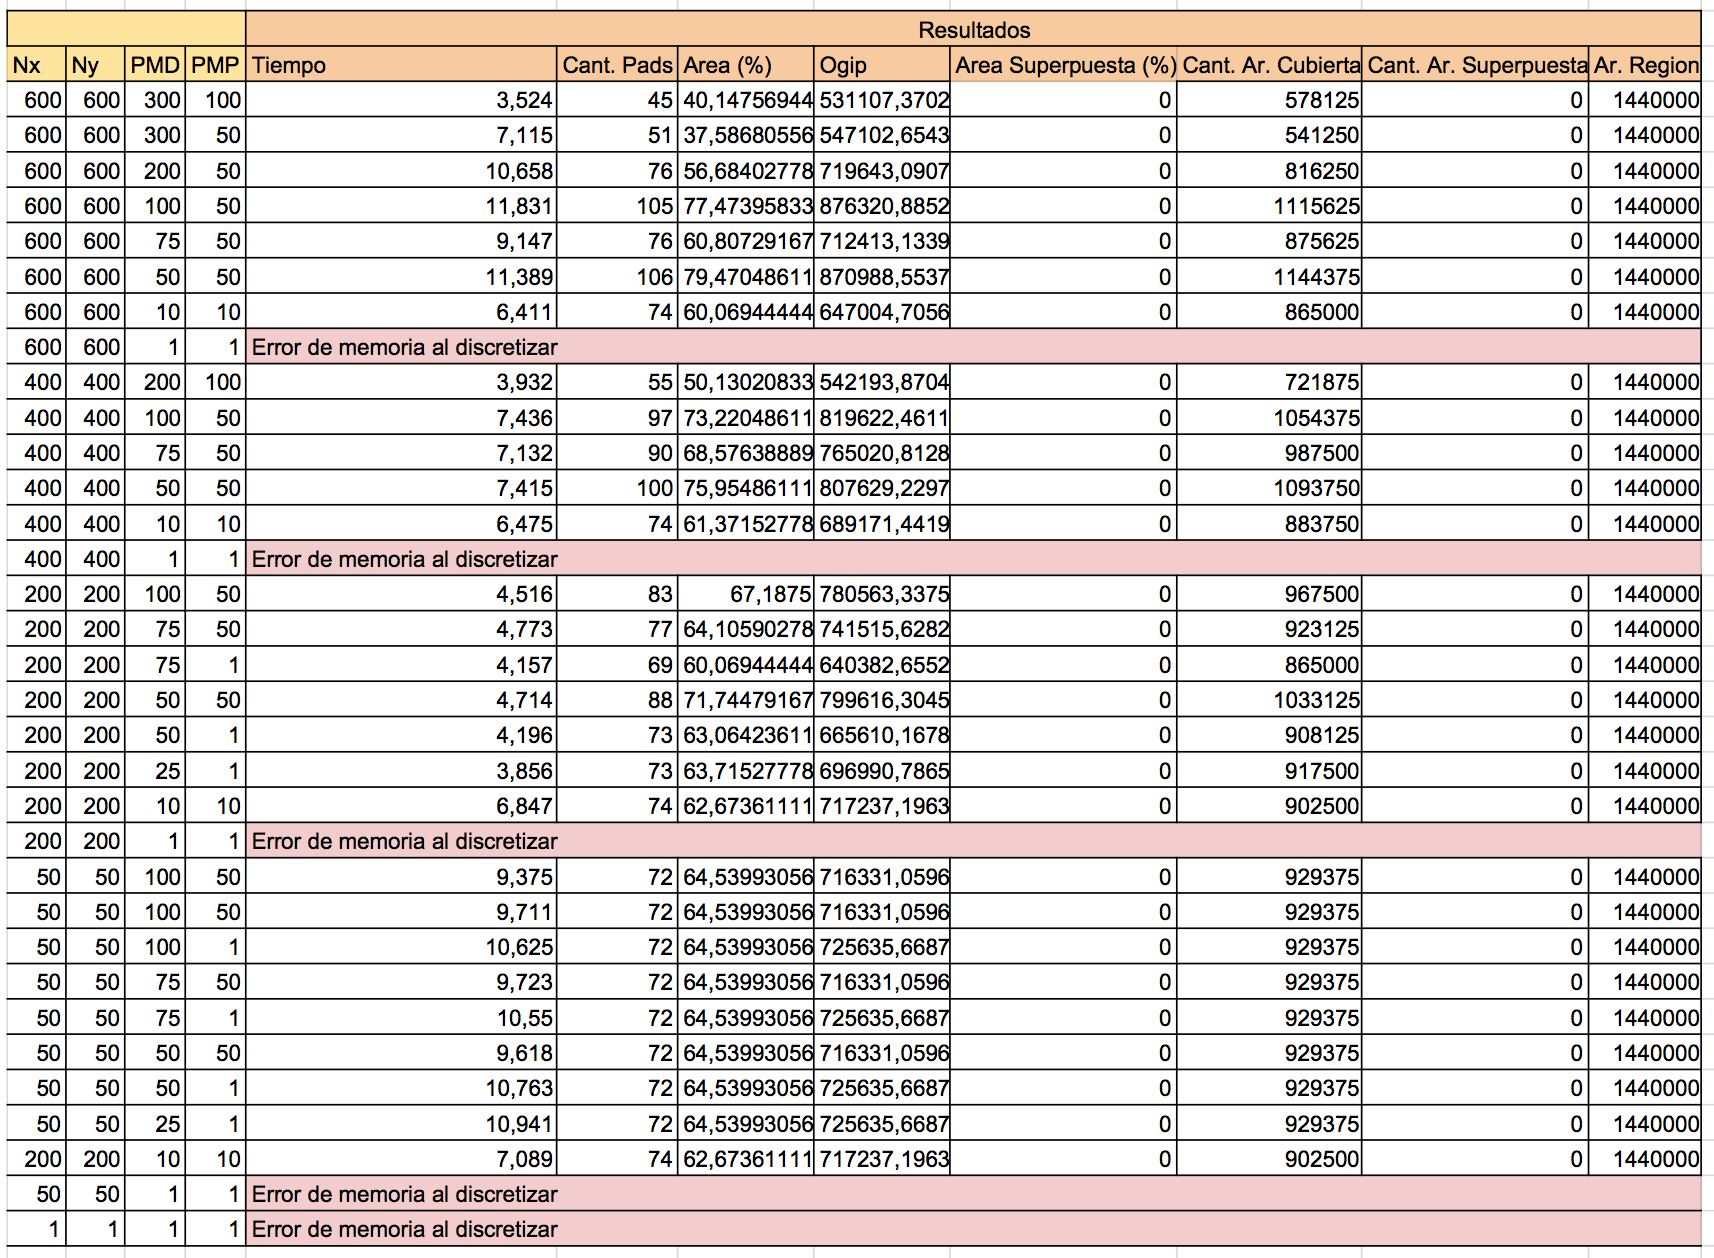
\includegraphics[width=1\textwidth]{imagenes/GML_0G1200x1200_muchos}
\end{center}

\subsection{45G1200x1200\_muchos}

\begin{center}
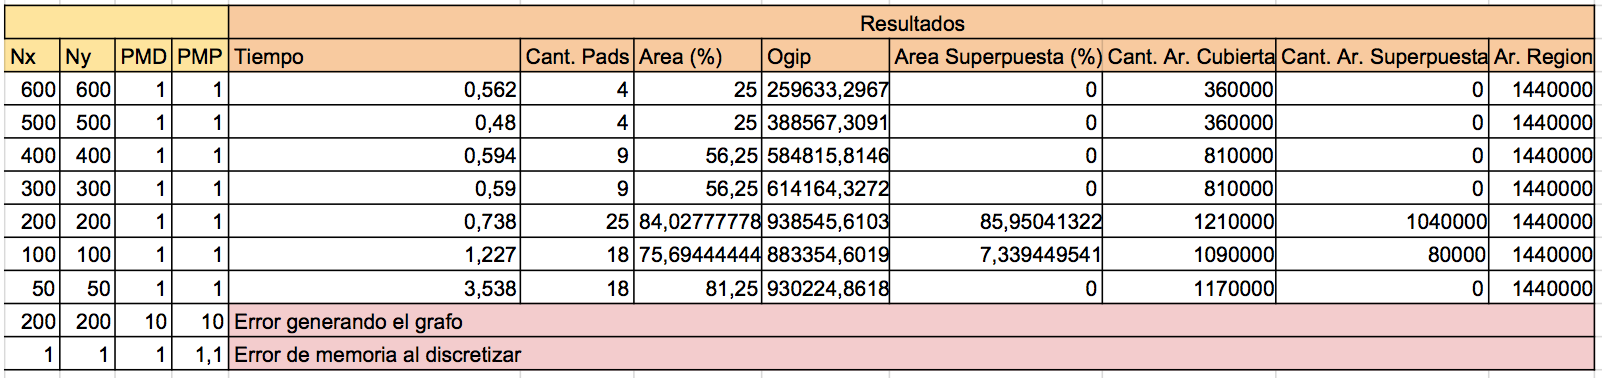
\includegraphics[width=1\textwidth]{imagenes/S_45G1200x1200_muchos}
\end{center}

\begin{center}
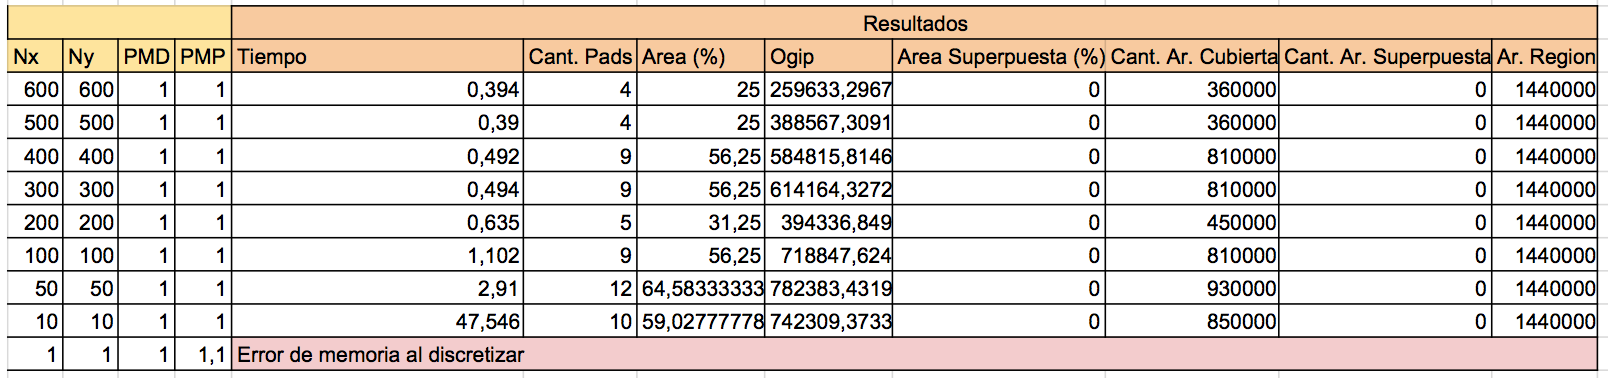
\includegraphics[width=1\textwidth]{imagenes/G_45G1200x1200_muchos}
\end{center}

\begin{center}
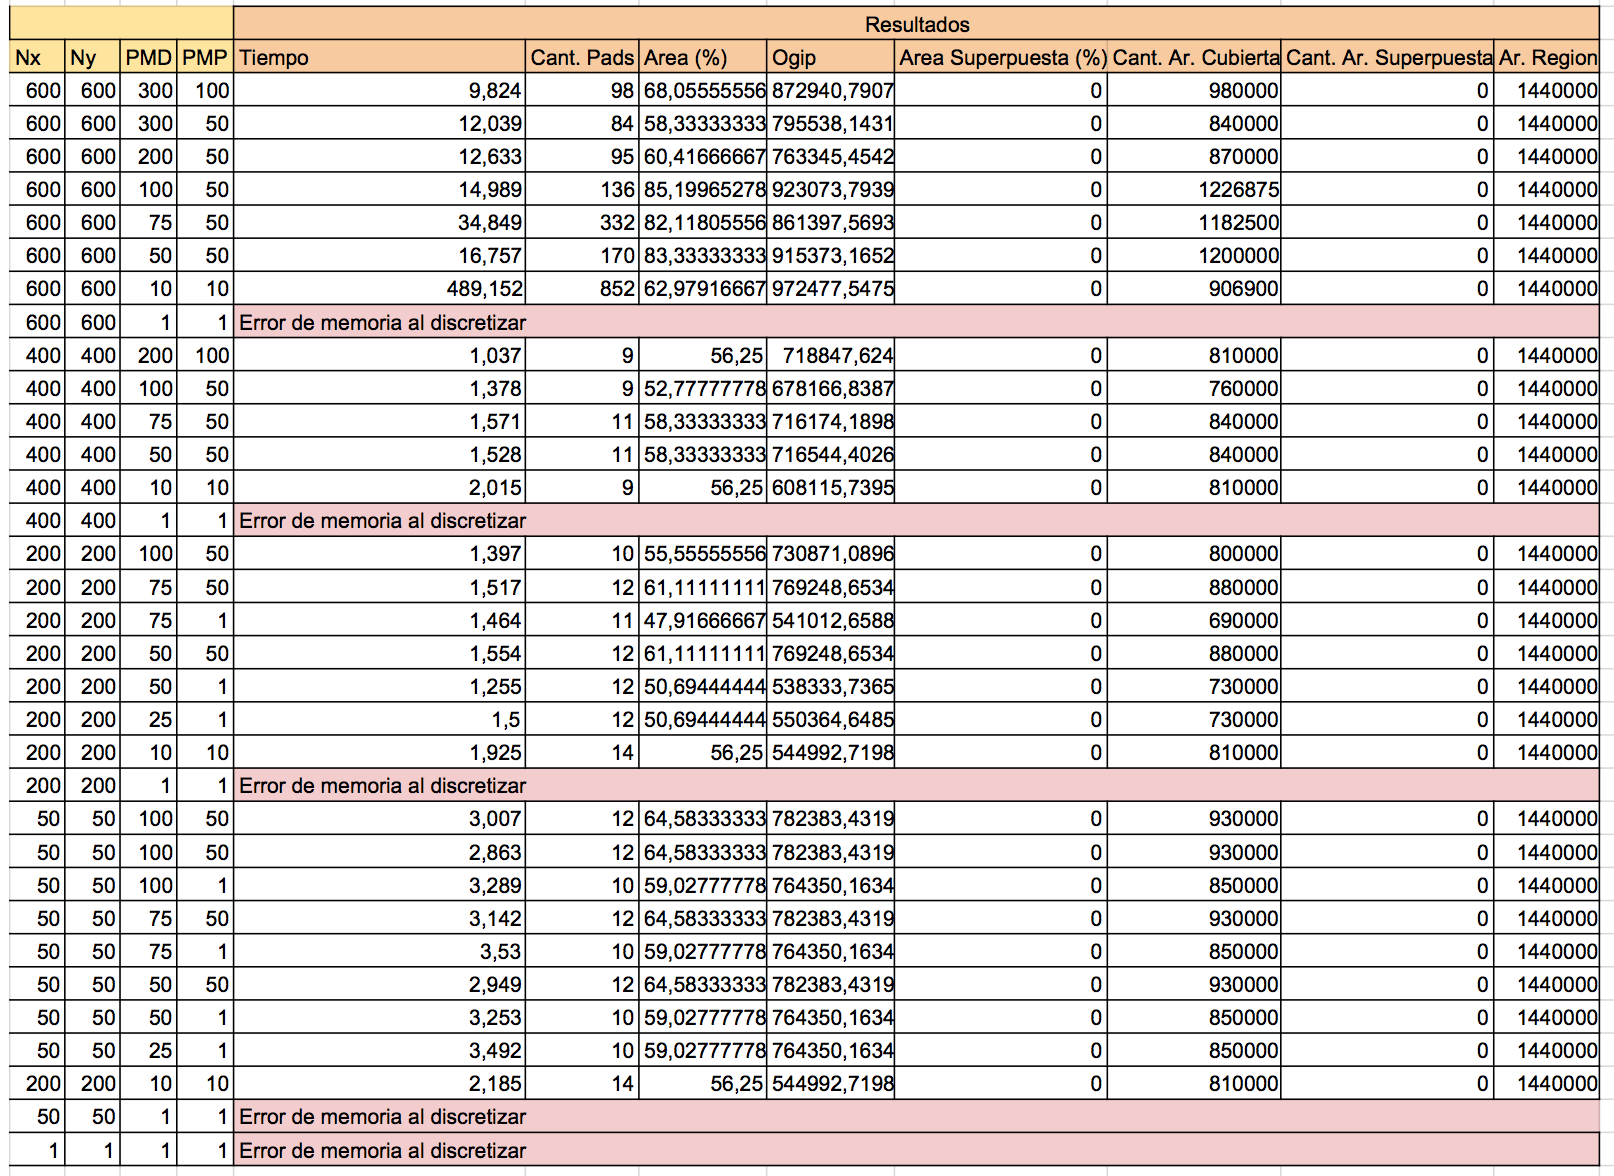
\includegraphics[width=1\textwidth]{imagenes/GML_45G1200x1200_muchos}
\end{center}


\subsection{45G110X90Y8E7AR}

\begin{center}
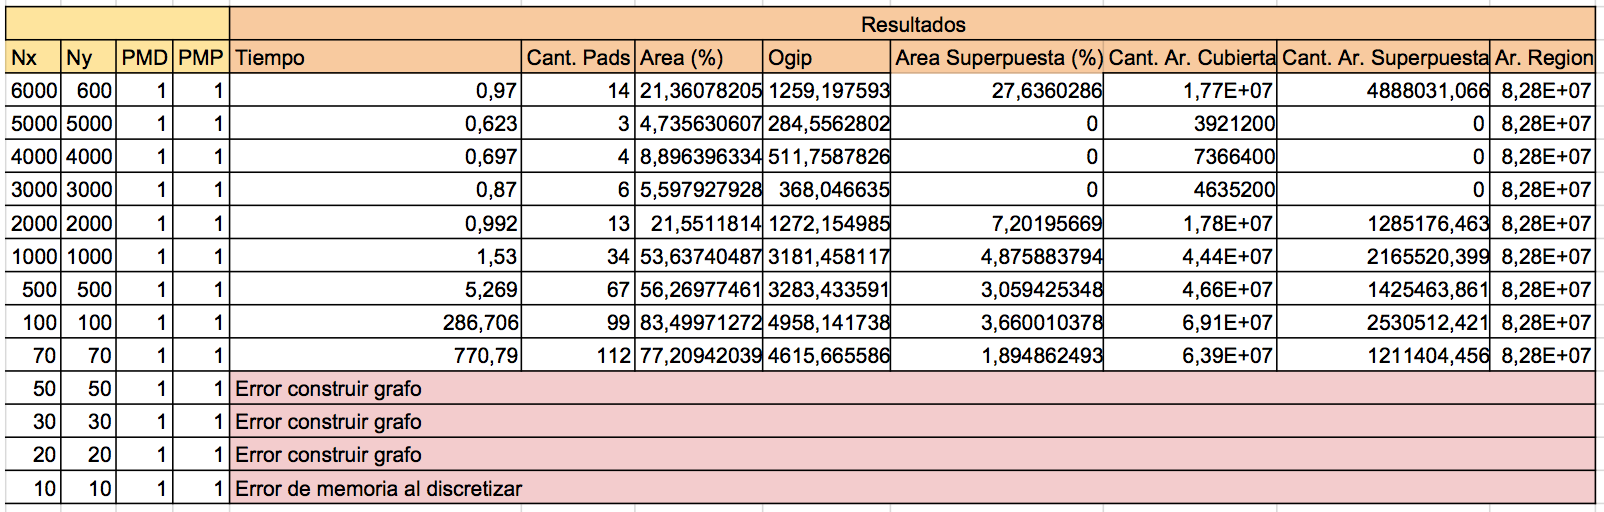
\includegraphics[width=1\textwidth]{imagenes/S_45G110X90Y8E7AR}
\end{center}

\begin{center}
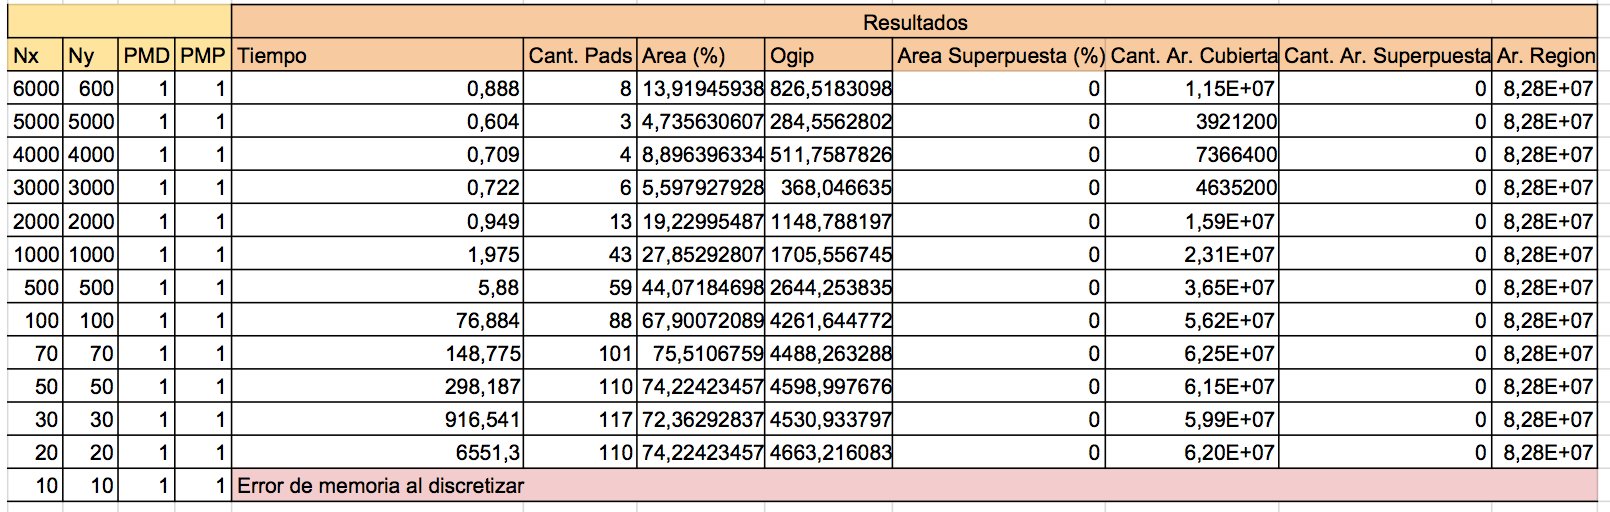
\includegraphics[width=1\textwidth]{imagenes/G_45G110X90Y8E7AR}
\end{center}

\begin{center}
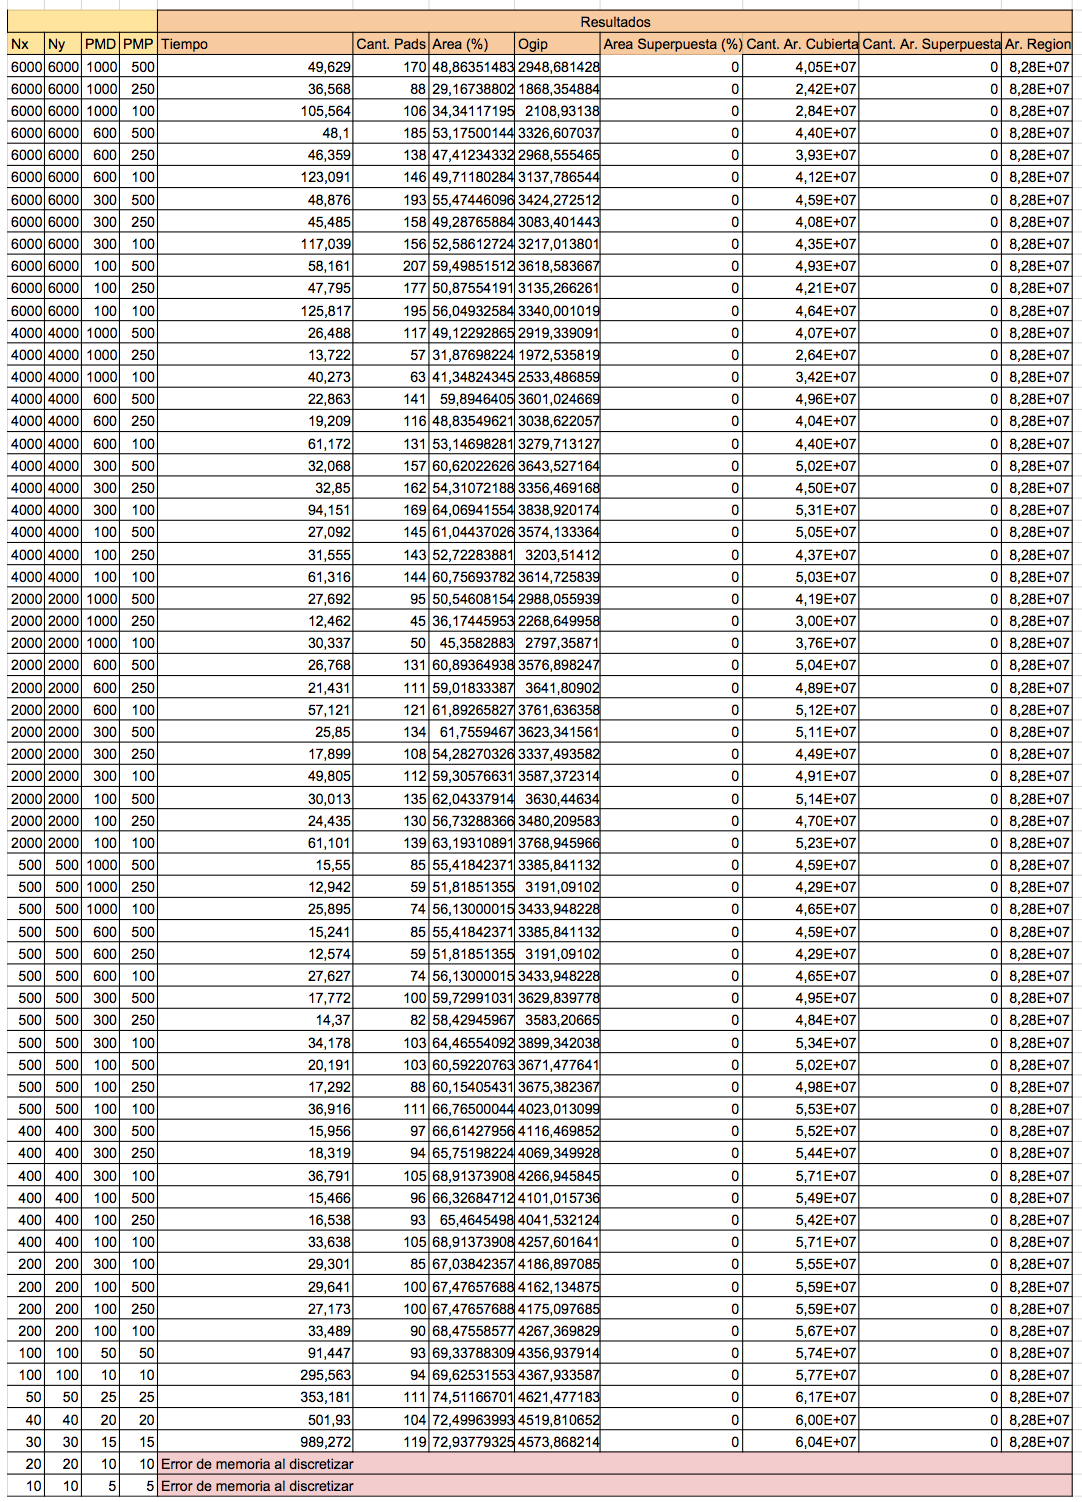
\includegraphics[width=1\textwidth]{imagenes/GML_45G110X90Y8E7AR}
\end{center}

